\documentclass{rapportECL}
\usepackage{lipsum}

% Packages pour couleurs et graphiques
\usepackage[utf8]{inputenc}
\usepackage[T1]{fontenc}
\usepackage[french]{babel}
\usepackage{geometry}
\usepackage{setspace}
\usepackage{hyperref}
\usepackage{xcolor}
\usepackage{tikz}
\usepackage{pgfplots}
\pgfplotsset{compat=1.18}
\usepackage{graphicx}
\usepackage{float}
\usepackage{booktabs}
\usepackage{array}
\usepackage{multirow}
\usepackage{colortbl}
\usepackage{fancyhdr}
\usepackage{tcolorbox}
\tcbuselibrary{breakable,skins}
\usepackage{enumitem}
\usepackage{amsmath}
\usepackage{amssymb}
\usepackage{listings}
\usepackage{caption}
\usepackage{subcaption}

% Configuration des couleurs
\definecolor{primaryblue}{RGB}{102, 126, 234}
\definecolor{secondarypurple}{RGB}{118, 75, 162}
\definecolor{accentgreen}{RGB}{16, 185, 129}
\definecolor{accentorange}{RGB}{245, 158, 11}
\definecolor{accentred}{RGB}{239, 68, 68}
\definecolor{lightgray}{RGB}{248, 249, 250}
\definecolor{darkgray}{RGB}{75, 85, 99}
\definecolor{textgray}{RGB}{107, 114, 128}

% Configuration hyperref
\hypersetup{
    colorlinks=true,
    linkcolor=primaryblue,
    filecolor=primaryblue,
    urlcolor=primaryblue,
    citecolor=primaryblue,
    pdftitle={Système Multi-Agents pour la Sélection Intelligente des Candidats},
    pdfauthor={Laila Ait Bihi, Chaima AL Ayachi, Salma Bouchama, Chaymae Dahhassi}
}

% Configuration des listings
\lstset{
    language=Python,
    basicstyle=\ttfamily\small,
    keywordstyle=\color{primaryblue}\bfseries,
    commentstyle=\color{textgray}\itshape,
    stringstyle=\color{accentgreen},
    numbers=left,
    numberstyle=\tiny\color{darkgray},
    stepnumber=1,
    numbersep=5pt,
    backgroundcolor=\color{lightgray},
    showspaces=false,
    showstringspaces=false,
    showtabs=false,
    frame=single,
    rulecolor=\color{primaryblue},
    tabsize=2,
    captionpos=b,
    breaklines=true,
    breakatwhitespace=false
}

% Style des tcolorbox
\newtcolorbox{infobox}[1]{
    colback=lightgray,
    colframe=primaryblue,
    title=#1,
    fonttitle=\bfseries\color{primaryblue},
    breakable,
    enhanced
}

\newtcolorbox{successbox}{
    colback=accentgreen!10,
    colframe=accentgreen,
    breakable,
    enhanced
}

\newtcolorbox{warningbox}{
    colback=accentorange!10,
    colframe=accentorange,
    breakable,
    enhanced
}

\newtcolorbox{importantbox}{
    colback=primaryblue!10,
    colframe=primaryblue,
    breakable,
    enhanced
}

% Titre du rapport
\title{Rapport ECL - Système Multi-Agents pour la Sélection Intelligente des Candidats}

\begin{document}

%----------- Informations du rapport ---------
\titre{Système Multi-Agents pour la Sélection Intelligente des Candidats en Entreprise}
\enseignant{Youssef \textsc{Lamrani}}
\eleves{Laila \textsc{Ait Bihi} \\
        Chaima \textsc{AL Ayachi}\\
        Salma \textsc{Bouchama} \\ 
        Chaymae \textsc{Dahhassi}}

%----------- Initialisation -------------------
\fairemarges
\fairepagedegarde
\tabledematieres

\onehalfspacing

%------------ Corps du rapport ----------------

\part{Introduction}

\section{Introduction}

\subsection{Contexte et Problématique}

Le recrutement moderne fait face à des défis majeurs qui impactent l'efficacité et l'équité du processus de sélection. Les entreprises sont confrontées à :

\begin{itemize}[leftmargin=*]
    \item \textbf{Volume croissant de candidatures} : Des centaines à milliers de CVs par poste à analyser
    \item \textbf{Coût temporel élevé} : 6-8 minutes en moyenne par CV pour une analyse approfondie
    \item \textbf{Subjectivité dans l'évaluation} : Biais cognitifs (effet de halo, biais de confirmation, etc.)
    \item \textbf{Manque de transparence} : Décisions difficiles à justifier et à expliquer
    \item \textbf{Difficulté d'identification} : Problème de trouver rapidement les meilleurs profils parmi un large vivier
\end{itemize}

\begin{importantbox}
\textbf{Enjeu majeur} : Selon une étude récente, 75\% des recruteurs estiment que le processus de sélection actuel est trop long et manque d'objectivité. Notre solution vise à transformer ce processus en le rendant plus rapide, plus objectif et entièrement explicable.
\end{importantbox}

\subsection{Objectifs du Projet}

Ce projet vise à développer un système intelligent et explicable de sélection de candidats qui :

\begin{enumerate}[leftmargin=*]
    \item \textbf{Automatise l'analyse} : Traitement automatique des documents de candidature (CVs, lettres de motivation)
    \item \textbf{Évalue objectivement} : Évaluation multidimensionnelle selon des critères clairs et mesurables
    \item \textbf{Fournit des justifications} : Explications détaillées et transparentes pour chaque décision
    \item \textbf{Simule un comité} : Architecture multi-agents reproduisant la dynamique d'un comité de recrutement
    \item \textbf{Offre une interface interactive} : Plateforme web intuitive pour les recruteurs
\end{enumerate}

\subsection{Innovation et Valeur Ajoutée}

Notre solution se distingue par plusieurs innovations clés :

\begin{tcolorbox}[colback=accentgreen!10,colframe=accentgreen,title=\textbf{Points d'Innovation}]
\begin{itemize}[leftmargin=*]
    \item \textbf{Architecture Multi-Agents avec CrewAI} : Simulation d'un comité d'experts où chaque agent a une spécialité (RH, Technique, Soft Skills, Profil, Décision)
    \item \textbf{Système RAG avancé} : Recherche sémantique pour une présélection intelligente basée sur la compréhension du sens, pas seulement les mots-clés
    \item \textbf{Explicabilité native} : Chaque décision est accompagnée d'une justification générée par LLM, respectant les principes de XAI (Explainable AI)
    \item \textbf{Approche holistique} : Évaluation simultanée des dimensions technique, comportementale et culturelle
    \item \textbf{Interface Streamlit moderne} : Expérience utilisateur soignée avec visualisations interactives et design professionnel
\end{itemize}
\end{tcolorbox}

\newpage

\part{Fondements Théoriques}

Une compréhension solide des concepts théoriques sous-jacents est essentielle pour appréhender les choix d'architecture et de technologie qui structurent ce système. Cette section sert de socle de connaissances, non seulement pour justifier la conception actuelle, mais aussi pour guider les ingénieurs qui seront chargés de la maintenance ou de l'évolution future du projet.

\section{Les Systèmes Multi-Agents (SMA)}

\subsection{Concepts Fondamentaux}

Un système multi-agents (SMA) est un paradigme informatique où plusieurs agents autonomes et intelligents interagissent dans un environnement commun pour résoudre des problèmes qui dépassent leurs capacités individuelles. 

\begin{infobox}{Caractéristiques d'un Agent}
Un agent dans un SMA possède quatre propriétés fondamentales :
\begin{itemize}
    \item \textbf{Autonomie} : Capacité à prendre des décisions indépendantes sans intervention humaine directe
    \item \textbf{Réactivité} : Capacité à percevoir l'environnement et réagir aux changements
    \item \textbf{Proactivité} : Capacité à initier des actions pour atteindre ses objectifs
    \item \textbf{Socialité} : Capacité à communiquer et collaborer avec d'autres agents
\end{itemize}
\end{infobox}

L'avantage de cette approche pour une tâche complexe comme le recrutement est sa capacité à décomposer le problème en sous-tâches spécialisées. Le système simule ainsi un ``comité virtuel'' où chaque agent évalue les candidats sous un angle différent (technique, humain, cohérence du profil), reflétant la dynamique d'un véritable comité de recrutement.

\subsection{Architecture Hiérarchique}

Notre système utilise une architecture hiérarchique illustrée dans la figure~\ref{fig:architecture_agents}.

\begin{figure}[H]
\centering
\begin{tikzpicture}[
    agent/.style={rectangle, rounded corners, draw=primaryblue, fill=primaryblue!10, 
                  text width=2.5cm, text centered, minimum height=1cm, font=\small},
    decideur/.style={rectangle, rounded corners, draw=accentgreen, fill=accentgreen!10,
                     text width=3cm, text centered, minimum height=1.2cm, font=\bfseries}
]
    % Agent Décideur
    \node[decideur] (decideur) at (0,0) {Agent Décideur};
    
    % Agents spécialisés
    \node[agent] (rh) at (-4,-2.5) {Agent RH};
    \node[agent] (profil) at (-1.5,-2.5) {Agent Profil};
    \node[agent] (tech) at (1.5,-2.5) {Agent Technique};
    \node[agent] (soft) at (4,-2.5) {Agent Soft Skills};
    
    % Flèches
    \draw[->, thick, primaryblue] (rh) -- (decideur);
    \draw[->, thick, primaryblue] (profil) -- (decideur);
    \draw[->, thick, primaryblue] (tech) -- (decideur);
    \draw[->, thick, primaryblue] (soft) -- (decideur);
\end{tikzpicture}
\caption{Architecture hiérarchique du système multi-agents}
\label{fig:architecture_agents}
\end{figure}

\subsection{Le Framework CrewAI}

Pour l'implémentation de cette logique agentique, le framework \textbf{CrewAI} a été choisi pour plusieurs raisons :

\begin{itemize}[leftmargin=*]
    \item \textbf{Définition déclarative} : Création d'agents en définissant simplement leurs rôles, objectifs et outils
    \item \textbf{Orchestration automatique} : Gestion automatique des interactions entre agents
    \item \textbf{Mémoire partagée} : Les agents peuvent partager des informations via un contexte commun
    \item \textbf{Intégration native LLM} : Support direct des grands modèles de langage via LangChain
    \item \textbf{Exécution séquentielle ou parallèle} : Flexibilité dans l'ordre d'exécution des tâches
\end{itemize}

\section{La Génération Augmentée par la Récupération (RAG)}

\subsection{Principe et Architecture}

La génération augmentée par la récupération (RAG) est une technique qui enrichit les capacités des grands modèles de langage (LLM) en leur donnant accès à une base de connaissances externe. 

Le RAG combine récupération d'information et génération de texte pour améliorer les LLMs. Le processus comprend trois phases principales :

\begin{enumerate}[leftmargin=*]
    \item \textbf{Indexation} : Conversion des documents en embeddings vectoriels
    \item \textbf{Récupération} : Recherche des documents les plus pertinents via similarité sémantique
    \item \textbf{Augmentation-Génération} : Enrichissement du contexte du LLM avec les documents récupérés, puis génération de la réponse
\end{enumerate}

\subsection{Formalisation Mathématique}

\textbf{Formule probabiliste du RAG :}
\begin{equation}
P(y | q) = \sum_{d \in \mathcal{C}} P(y | q, d) \cdot P(d | q)
\end{equation}

où :
\begin{itemize}
    \item $q$ est la requête (description de poste)
    \item $y$ est la réponse générée
    \item $d$ est un document de la collection $\mathcal{C}$
    \item $P(d | q)$ est la probabilité de récupération du document $d$ étant donné $q$
    \item $P(y | q, d)$ est la probabilité de génération de $y$ étant donné $q$ et $d$
\end{itemize}

\textbf{Embeddings sémantiques :} Nous utilisons le modèle \texttt{all-MiniLM-L6-v2} (384 dimensions, architecture Transformer 6 couches). La similarité est calculée via distance cosinus :

\begin{equation}
\text{sim}(t_1, t_2) = \frac{\mathbf{e}_1 \cdot \mathbf{e}_2}{\|\mathbf{e}_1\| \|\mathbf{e}_2\|} = \cos(\theta)
\end{equation}

où $\mathbf{e}_1$ et $\mathbf{e}_2$ sont les embeddings vectoriels des textes $t_1$ et $t_2$, et $\theta$ est l'angle entre ces vecteurs.

\subsection{Application dans le Projet}

Dans ce projet, le RAG est appliqué pour effectuer une présélection intelligente : une base de données vectorielle est utilisée pour rechercher et extraire les CVs et documents les plus pertinents par rapport aux exigences formulées dans une description de poste. 

\begin{infobox}{Technologies RAG Implémentées}
\begin{itemize}
    \item \textbf{ChromaDB} : Base de données vectorielle persistante avec index HNSW (Hierarchical Navigable Small World) pour recherche rapide
    \item \textbf{Embeddings all-MiniLM-L6-v2} : Modèle de transformation texte-vecteur optimisé pour la vitesse et la qualité
    \item \textbf{Similarité cosinus} : Métrique de distance pour mesurer la pertinence sémantique
\end{itemize}
\end{infobox}

En ancrant le raisonnement des agents sur des extraits de CV pertinents et factuels, le RAG agit comme un garde-fou contre les hallucinations du LLM, garantissant que les évaluations sont fondées sur les données réelles du candidat.

\section{Traitement du Langage Naturel (NLP)}

\subsection{Named Entity Recognition (NER)}

La reconnaissance d'entités nommées (Named Entity Recognition) consiste à identifier et classifier automatiquement des entités sémantiques présentes dans un texte. Dans ce projet, nous utilisons la bibliothèque \texttt{spaCy} avec le modèle pré-entraîné \texttt{fr\_core\_news\_sm}, spécifiquement conçu pour le traitement du langage naturel en français.

Ce modèle permet l'extraction des principales catégories d'entités :

\begin{table}[H]
\centering
\begin{tabular}{ll}
\toprule
\textbf{Type d'Entité} & \textbf{Exemples} \\
\midrule
\texttt{PERSON} & Noms de personnes, candidats, références \\
\texttt{ORG} & Organisations, entreprises, universités \\
\texttt{LOC} & Lieux géographiques, villes, pays \\
\texttt{DATE} & Expressions temporelles, périodes d'emploi \\
\bottomrule
\end{tabular}
\caption{Types d'entités extraites par le modèle NER}
\label{tab:ner_entities}
\end{table}

D'un point de vue architectural, le modèle repose sur un réseau de neurones convolutionnel (CNN) combiné à un parseur transitionnel. L'annotation des entités suit le schéma \textbf{BIO} (\textit{Begin-Inside-Outside}), dans lequel chaque token est étiqueté selon sa position au sein d'une entité nommée.

\begin{infobox}{Performance du Modèle NER}
En termes de performance, le modèle \texttt{fr\_core\_news\_sm} atteint un \textbf{F1-score d'environ 84\%} sur des benchmarks de référence en langue française, ce qui témoigne d'un bon compromis entre précision et rappel pour des tâches d'extraction d'information en contexte réel.
\end{infobox}

\subsection{Extraction de Compétences}

L'extraction de compétences utilise une méthode hybride :

\begin{itemize}[leftmargin=*]
    \item \textbf{Dictionnaire prédéfini} : Base de connaissances avec 30+ compétences techniques (Python, Machine Learning, SQL, etc.) et 15+ soft skills (Communication, Leadership, etc.)
    \item \textbf{Matching case-insensitive} : Recherche insensible à la casse pour capturer les variations
    \item \textbf{Contexte sémantique} : Analyse du contexte d'utilisation pour éviter les faux positifs
\end{itemize}

\subsection{Extraction d'Expérience}

L'extraction des années d'expérience utilise des expressions régulières pour détecter les patterns temporels :

\begin{lstlisting}[caption=Exemple d'extraction d'expérience, label=lst:experience_extraction]
# Patterns détectés
"expérience de X ans"
"X années d'expérience"
"depuis X ans"
"X ans dans le domaine"
\end{lstlisting}

\section{Modèles de Langage (LLM)}

\subsection{Architecture Transformer}

Au cœur du système se trouvent les grands modèles de langage (LLM), qui fournissent les capacités de raisonnement et de compréhension du langage. Ce projet s'appuie sur le modèle \textbf{Llama 3.3 70B} via l'API Groq pour bénéficier d'une inférence ultra-rapide (500+ tokens/s).

\begin{table}[H]
\centering
\begin{tabular}{ll}
\toprule
\textbf{Caractéristique} & \textbf{Valeur} \\
\midrule
Paramètres & 70 milliards \\
Fenêtre contextuelle & 8192 tokens \\
Entraînement & 15 trillions de tokens \\
Vitesse d'inférence & 500+ tokens/s (Groq) \\
Architecture & Transformer (attention multi-têtes) \\
\bottomrule
\end{tabular}
\caption{Spécifications du modèle Llama 3.3 70B}
\label{tab:llm_specs}
\end{table}

\subsection{Rôle dans le Système}

Chaque agent utilise le LLM pour :
\begin{itemize}[leftmargin=*]
    \item Analyser les informations qui lui sont fournies (fragments de CV, description de poste)
    \item Évaluer les candidats selon ses critères spécifiques
    \item Générer des justifications textuelles claires et explicables
    \item Produire des sorties structurées (JSON) pour faciliter le traitement automatique
\end{itemize}

\begin{importantbox}
\textbf{Avantage Groq} : L'utilisation de l'API Groq permet d'obtenir des réponses en temps réel (latence < 2 secondes) même avec un modèle de 70B paramètres, rendant l'expérience utilisateur fluide et interactive.
\end{importantbox}

\newpage

\part{Données, Architecture et Implémentation du Système}

Cette section constitue le cœur de ce rapport technique. Elle décompose l'architecture globale du système en ses modules principaux, décrivant en détail le rôle de chaque composant, les technologies utilisées et la logique d'interaction qui les unit pour former un pipeline de traitement cohérent et efficace.

\section{Données utilisées}

\subsection{Description des données}

Notre dataset comprend :

\begin{itemize}[leftmargin=*]
    \item \textbf{Documents candidats} : CVs en formats PDF/DOCX/TXT (500-1500 mots par document)
    \item \textbf{Descriptions de postes} : Fichiers .txt structurés contenant les exigences et critères de sélection
\end{itemize}

\subsection{Statistiques du Dataset}

Sur un échantillon de 10 candidats analysés, nous avons obtenu les statistiques suivantes :

\begin{table}[H]
\centering
\begin{tabular}{lcc}
\toprule
\textbf{Métrique} & \textbf{Moyenne} & \textbf{Écart-type} \\
\midrule
Mots par CV & 852 & 234 \\
Phrases par CV & 38 & 12 \\
Compétences techniques & 4.2 & 1.8 \\
Soft skills & 2.8 & 1.2 \\
Années d'expérience & 3.4 & 2.1 \\
\bottomrule
\end{tabular}
\caption{Statistiques descriptives du dataset}
\label{tab:dataset_stats}
\end{table}

\subsection{Analyse Exploratoire}

\textbf{Distribution des compétences :} Les trois compétences techniques les plus fréquentes sont :
\begin{enumerate}[leftmargin=*]
    \item Python (70\% des candidats)
    \item Machine Learning (50\% des candidats)
    \item SQL (40\% des candidats)
\end{enumerate}

\textbf{Distribution de l'expérience :} 
\begin{itemize}[leftmargin=*]
    \item Juniors (0-2 ans) : 30\%
    \item Confirmés (2-5 ans) : 50\%
    \item Seniors (5+ ans) : 20\%
\end{itemize}

\textbf{Corrélation :} Coefficient de Pearson $r=0.65$ entre expérience et longueur du CV (corrélation modérée positive), suggérant que les candidats plus expérimentés tendent à avoir des CVs plus détaillés.

\section{Architecture Globale et Modulaire}

Le projet est structuré selon une architecture modulaire, où chaque grande fonctionnalité est encapsulée dans son propre répertoire. Cette organisation favorise la séparation des préoccupations et rend le code plus facile à comprendre et à maintenir.

\begin{figure}[H]
\centering
\begin{tikzpicture}[
    module/.style={rectangle, rounded corners, draw=primaryblue, fill=primaryblue!10,
                  text width=3cm, text centered, minimum height=1cm},
    data/.style={rectangle, rounded corners, draw=accentgreen, fill=accentgreen!10,
                text width=2.5cm, text centered, minimum height=0.8cm},
    arrow/.style={->, thick, primaryblue}
]
    % Modules
    \node[module] (preproc) at (0,3) {Preprocessing};
    \node[module] (rag) at (3,3) {RAG};
    \node[module] (agents) at (6,3) {Agents};
    \node[module] (app) at (3,1) {Streamlit App};
    
    % Données
    \node[data] (raw) at (-2,3) {Raw Data};
    \node[data] (vector) at (3,4.5) {Vector DB};
    \node[data] (results) at (6,1) {Results};
    
    % Flèches
    \draw[arrow] (raw) -- (preproc);
    \draw[arrow] (preproc) -- (rag);
    \draw[arrow] (rag) -- (vector);
    \draw[arrow] (vector) -- (agents);
    \draw[arrow] (agents) -- (results);
    \draw[arrow] (app) -- (preproc);
    \draw[arrow] (app) -- (rag);
    \draw[arrow] (app) -- (agents);
\end{tikzpicture}
\caption{Architecture modulaire du système}
\label{fig:architecture_modulaire}
\end{figure}

Les principaux répertoires sont :
\begin{itemize}[leftmargin=*]
    \item \texttt{preprocessing/} : Prétraitement et analyse exploratoire
    \item \texttt{rag/} : Système RAG et base vectorielle
    \item \texttt{agents/} : Définition des agents spécialisés
    \item \texttt{utils/} : Configuration et utilitaires
\end{itemize}

\section{Module de Prétraitement et d'Analyse Exploratoire (EDA)}

Ce module est la première étape du pipeline et a pour fonction de préparer les données brutes des candidats pour les analyses ultérieures.

\subsection{Composants du Module}

\begin{enumerate}[leftmargin=*]
    \item \textbf{\texttt{data\_loader.py}} : Gère le chargement des CVs et lettres de motivation à partir de divers formats de fichiers (PDF, DOCX, TXT) et en extrait le contenu textuel brut.
    
    \item \textbf{\texttt{text\_processor.py}} : Prend en charge le nettoyage et la normalisation du texte. Il utilise la bibliothèque spaCy pour des tâches avancées comme l'extraction d'entités nommées (NER) et l'identification systématique des compétences techniques et interpersonnelles.
    
    \item \textbf{\texttt{exploratory\_analysis.py}} : Fournit des outils pour calculer des statistiques descriptives sur le corpus de candidats et générer des visualisations (avec matplotlib, seaborn et plotly) pour analyser, par exemple, la distribution des compétences.
\end{enumerate}

\section{Module RAG et Base de Données Vectorielle}

Ce module implémente le système de génération augmentée par la récupération (RAG) pour la présélection des candidats.

\subsection{Composants du Module}

\begin{itemize}[leftmargin=*]
    \item \textbf{\texttt{vector\_store.py}} : Gère l'intégration avec la base de données vectorielle ChromaDB. Il utilise les embeddings all-MiniLM-L6-v2 pour convertir le contenu textuel de chaque document candidat en un vecteur numérique dense. Ces vecteurs sont ensuite stockés et indexés à l'aide de l'algorithme HNSW (Hierarchical Navigable Small World), qui offre un compromis efficace entre vitesse de recherche et précision.
    
    \item \textbf{\texttt{retriever.py}} : Orchestre le processus de recherche. En se basant sur les exigences du poste, il interroge la base de données vectorielle pour identifier les candidats les plus pertinents via la similarité cosinus, une métrique qui mesure l'orientation plutôt que la magnitude des vecteurs, la rendant particulièrement efficace pour évaluer la pertinence sémantique indépendamment de la longueur du document.
\end{itemize}

\section{Le Système Multi-Agents avec CrewAI}

Le cœur du raisonnement du système est géré par une équipe d'agents spécialisés, développés et orchestrés à l'aide du framework CrewAI.

\subsection{Description des Agents}

\begin{enumerate}[leftmargin=*]
    \item \textbf{Agent RH (\texttt{hr\_agent.py})} : Cet agent est le point de départ du processus d'évaluation. Sa responsabilité est d'analyser en profondeur la description de poste fournie par le recruteur pour en extraire les critères essentiels (compétences techniques, niveau d'expérience, qualités humaines, etc.).
    
    \item \textbf{Agent Profil (\texttt{profile\_agent.py})} : Il se concentre sur le candidat dans sa globalité. En analysant le CV et la lettre de motivation, il évalue la cohérence du parcours professionnel, la progression de carrière et la pertinence générale du profil par rapport au secteur d'activité.
    
    \item \textbf{Agent Technique (\texttt{technical\_agent.py})} : Cet agent est le spécialiste technique de l'équipe. Il évalue spécifiquement les compétences techniques mentionnées par le candidat et les compare rigoureusement aux exigences techniques du poste.
    
    \item \textbf{Agent Soft Skills (\texttt{soft\_skills\_agent.py})} : Son rôle est d'analyser les aspects humains du candidat. Il recherche des indicateurs de qualités interpersonnelles (communication, travail d'équipe, etc.) et évalue l'adéquation culturelle potentielle avec l'entreprise.
    
    \item \textbf{Agent Décideur (\texttt{decider\_agent.py})} : C'est le chef d'orchestre final. Il a la tâche cruciale d'agréger les scores et les analyses produits par tous les autres agents. Sur cette base, il génère le classement final, rédige des justifications détaillées et explicables pour chaque classement, et compile le rapport final.
\end{enumerate}

\section{Orchestration du Workflow}

La coordination de l'ensemble de ces modules et agents est assurée par le script \texttt{candidate\_selection\_system.py}. Ce module agit comme le \textit{control plane} du système, garantissant un pipeline d'exécution déterministe et reproductible.

\begin{figure}[H]
\centering
\begin{tikzpicture}[
    step/.style={rectangle, rounded corners, draw=primaryblue, fill=primaryblue!10,
                 text width=2.5cm, text centered, minimum height=0.8cm},
    arrow/.style={->, thick, primaryblue}
]
    \node[step] (1) at (0,0) {1. Chargement};
    \node[step] (2) at (2.5,0) {2. Prétraitement};
    \node[step] (3) at (5,0) {3. RAG};
    \node[step] (4) at (7.5,0) {4. Évaluation};
    \node[step] (5) at (10,0) {5. Décision};
    
    \draw[arrow] (1) -- (2);
    \draw[arrow] (2) -- (3);
    \draw[arrow] (3) -- (4);
    \draw[arrow] (4) -- (5);
\end{tikzpicture}
\caption{Pipeline d'exécution du système}
\label{fig:pipeline}
\end{figure}

\section{Synthèse des Technologies}

Le tableau suivant synthétise la pile technologique utilisée pour la construction de ce système :

\begin{table}[H]
\centering
\begin{tabular}{ll}
\toprule
\textbf{Domaine} & \textbf{Technologies} \\
\midrule
Framework Agentique & CrewAI 0.22.0 \\
NLP & spaCy 3.7.2, Sentence-Transformers 2.2.2 \\
RAG & ChromaDB 0.4.24, all-MiniLM-L6-v2 \\
LLM & Groq API 0.4.2, Llama 3.3 70B \\
Interface & Streamlit 1.29.0 \\
Visualisation & Plotly 5.18.0, Matplotlib 3.8.2, Seaborn 0.13.0 \\
Traitement de Données & Pandas 2.1.3, NumPy 1.26.2 \\
XAI & SHAP 0.44.0 \\
\bottomrule
\end{tabular}
\caption{Pile technologique du système}
\label{tab:tech_stack}
\end{table}

\newpage

\part{Interface Utilisateur et Cas d'Usage}

Cette section est dédiée à la démonstration pratique du système. Elle décrit l'interface utilisateur développée avec Streamlit, qui sert de portail d'interaction pour le recruteur, et illustre le workflow complet du système à travers un scénario de recrutement réaliste.

\section{Présentation de l'Interface Streamlit}

L'application web, encapsulée dans le fichier \texttt{app.py}, constitue le point d'entrée unique et convivial pour l'utilisateur. Elle est conçue pour être intuitive et guider le recruteur à travers les différentes étapes du processus.

\subsection{Architecture de l'Interface}

L'interface est structurée en plusieurs pages ou onglets, chacun ayant une fonction précise :

\begin{enumerate}[leftmargin=*]
    \item \textbf{Page d'accueil} : Fournit une présentation générale du système, de ses objectifs et de son fonctionnement. Elle présente également l'architecture multi-agents de manière visuelle.
    
    \item \textbf{Page d'analyse exploratoire} : Cette page offre au recruteur une vue d'ensemble immédiate de son vivier de talents, lui permettant d'identifier les tendances et la distribution des compétences clés avant même de lancer une évaluation individuelle.
    
    \item \textbf{Page d'évaluation multi-agents} : C'est ici que le processus d'évaluation est initié. L'utilisateur peut saisir ou coller une description de poste complète, puis lancer l'analyse par le système multi-agents.
    
    \item \textbf{Page de résultats} : Plus qu'un simple classement, cette page est un véritable outil d'aide à la décision, fournissant des arguments qualitatifs et quantitatifs pour chaque candidat afin de faciliter et d'objectiver les débriefings de recrutement. Elle présente des visualisations interactives créées avec Plotly pour explorer les résultats.
\end{enumerate}

\subsection{Page d'Accueil}

La page d'accueil présente le système de manière professionnelle avec un design moderne utilisant des dégradés de couleurs et des cartes d'information.

\begin{figure}[H]
\centering

\includegraphics[width=0.95\linewidth]{screenshots plateforme/Page accueil streamlit 1.png}
\caption{Page d'accueil de l'interface Streamlit}
\label{fig:accueil1}
\end{figure}

\begin{figure}[H]
\centering
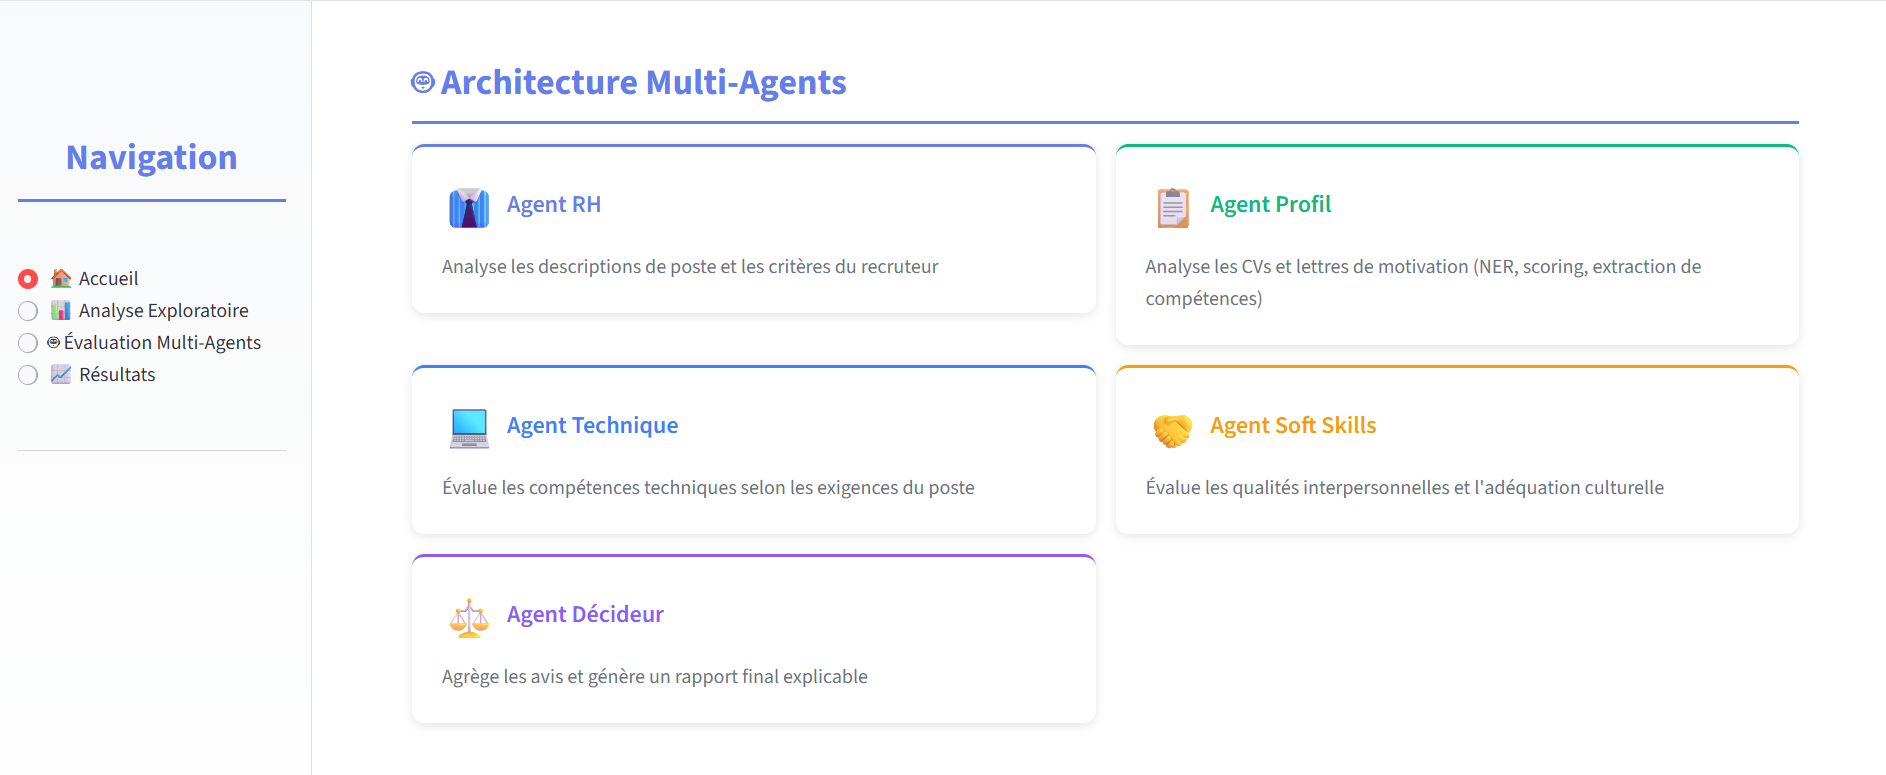
\includegraphics[width=0.95\linewidth]{screenshots plateforme/Page accueil streamlit 2.png}
\caption{Présentation de l'architecture multi-agents}
\label{fig:accueil2}
\end{figure}

\begin{figure}[H]
\centering
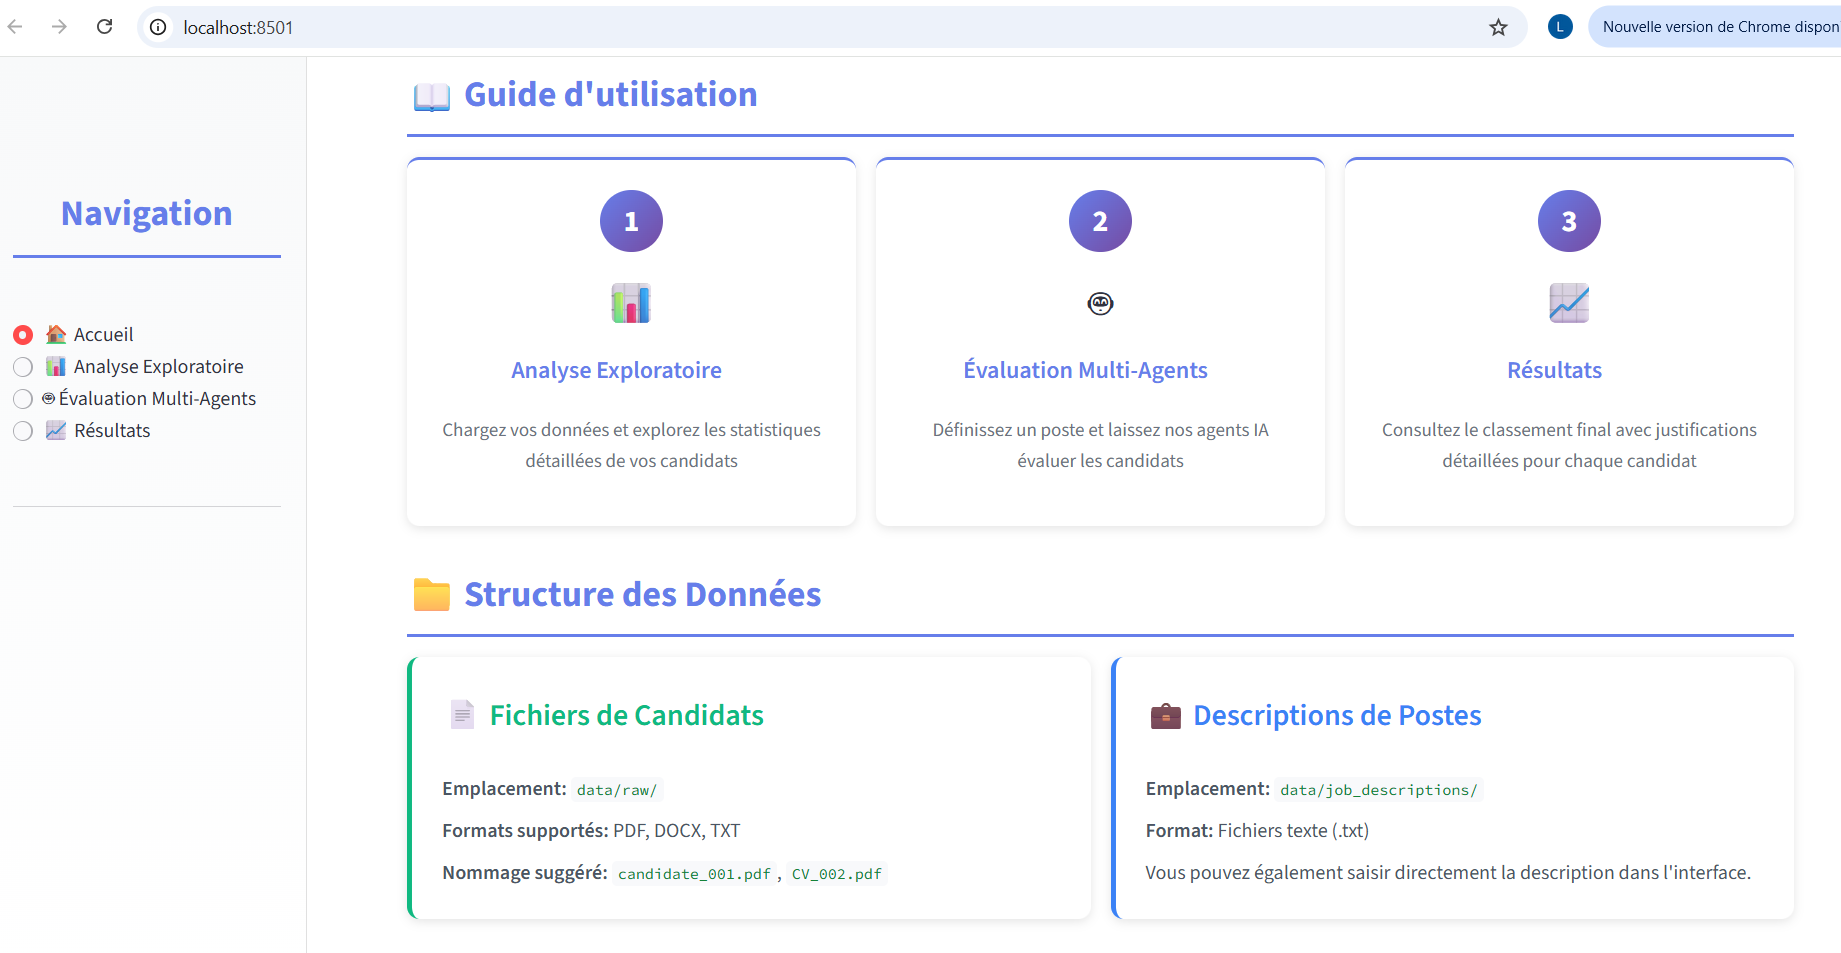
\includegraphics[width=0.95\linewidth]{screenshots plateforme/page accueil streamlit 3.png}
\caption{Guide d'utilisation en trois étapes}
\label{fig:accueil3}
\end{figure}

\begin{figure}[H]
\centering
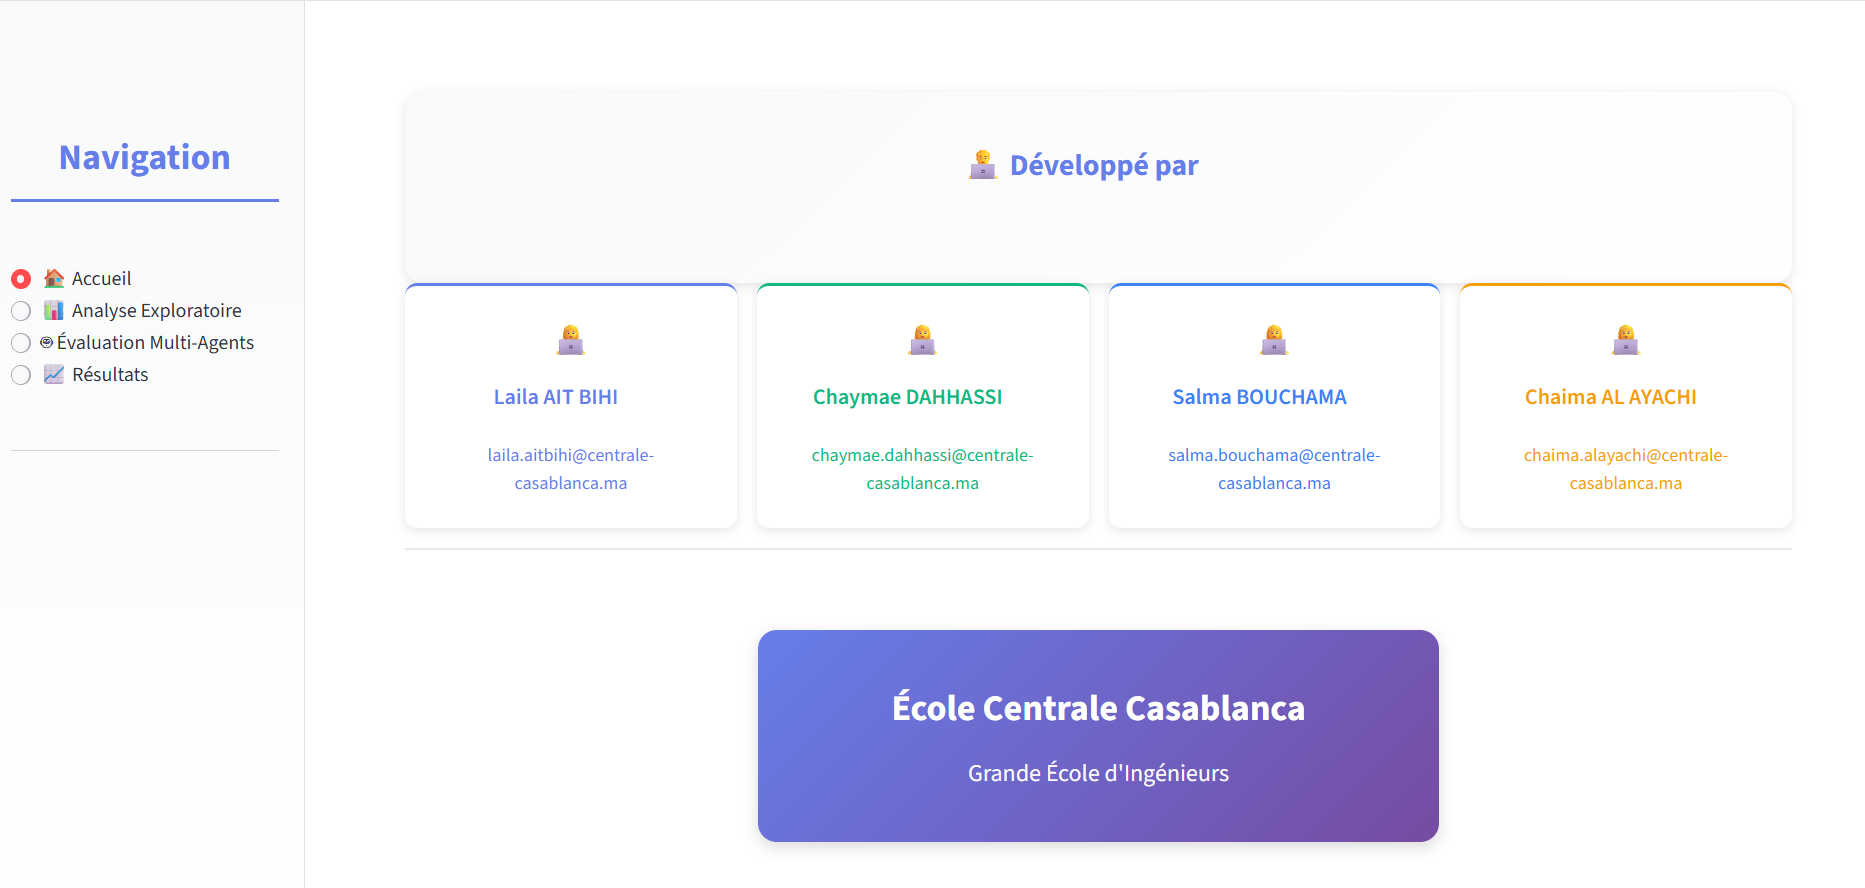
\includegraphics[width=0.95\linewidth]{screenshots plateforme/page accueil streamlit 4.png}
\caption{Informations sur la structure des données et crédits}
\label{fig:accueil4}
\end{figure}

\subsection{Page d'Analyse Exploratoire}

Cette page permet au recruteur de charger et analyser les candidats avant l'évaluation. Elle affiche des statistiques détaillées et des visualisations interactives.

\begin{figure}[H]
\centering
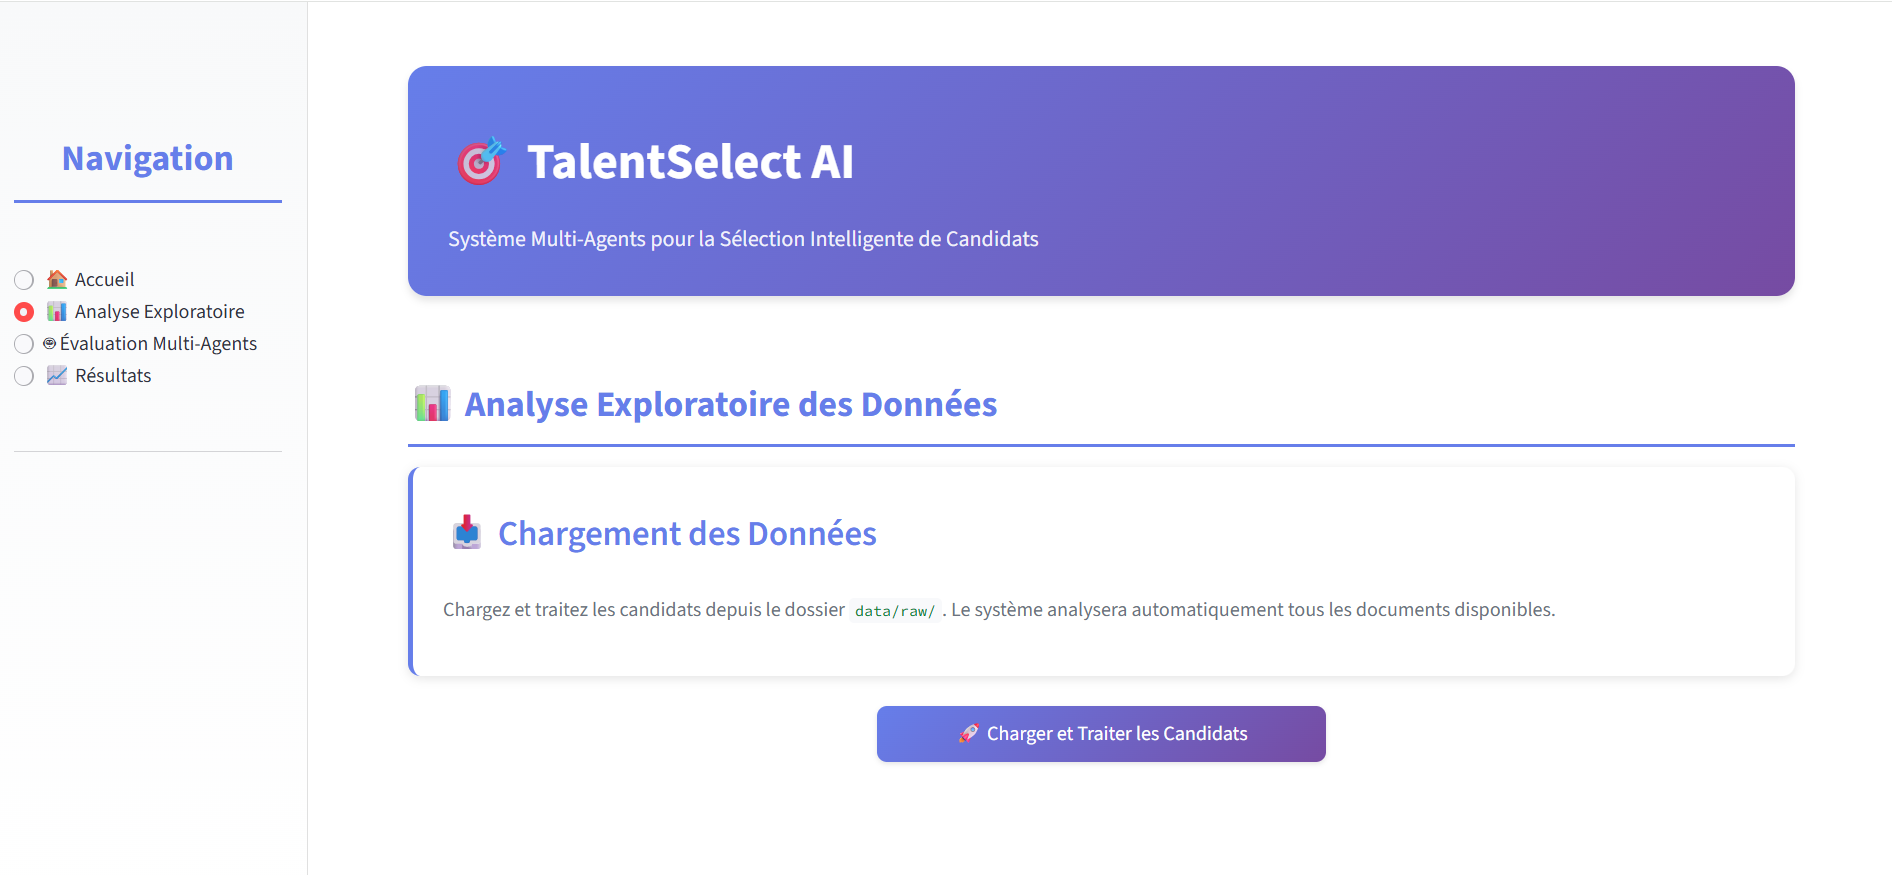
\includegraphics[width=0.95\linewidth]{screenshots plateforme/page analyse exploratoire streamlit 1.png}
\caption{Interface de chargement des candidats}
\label{fig:eda1}
\end{figure}

\begin{figure}[H]
\centering
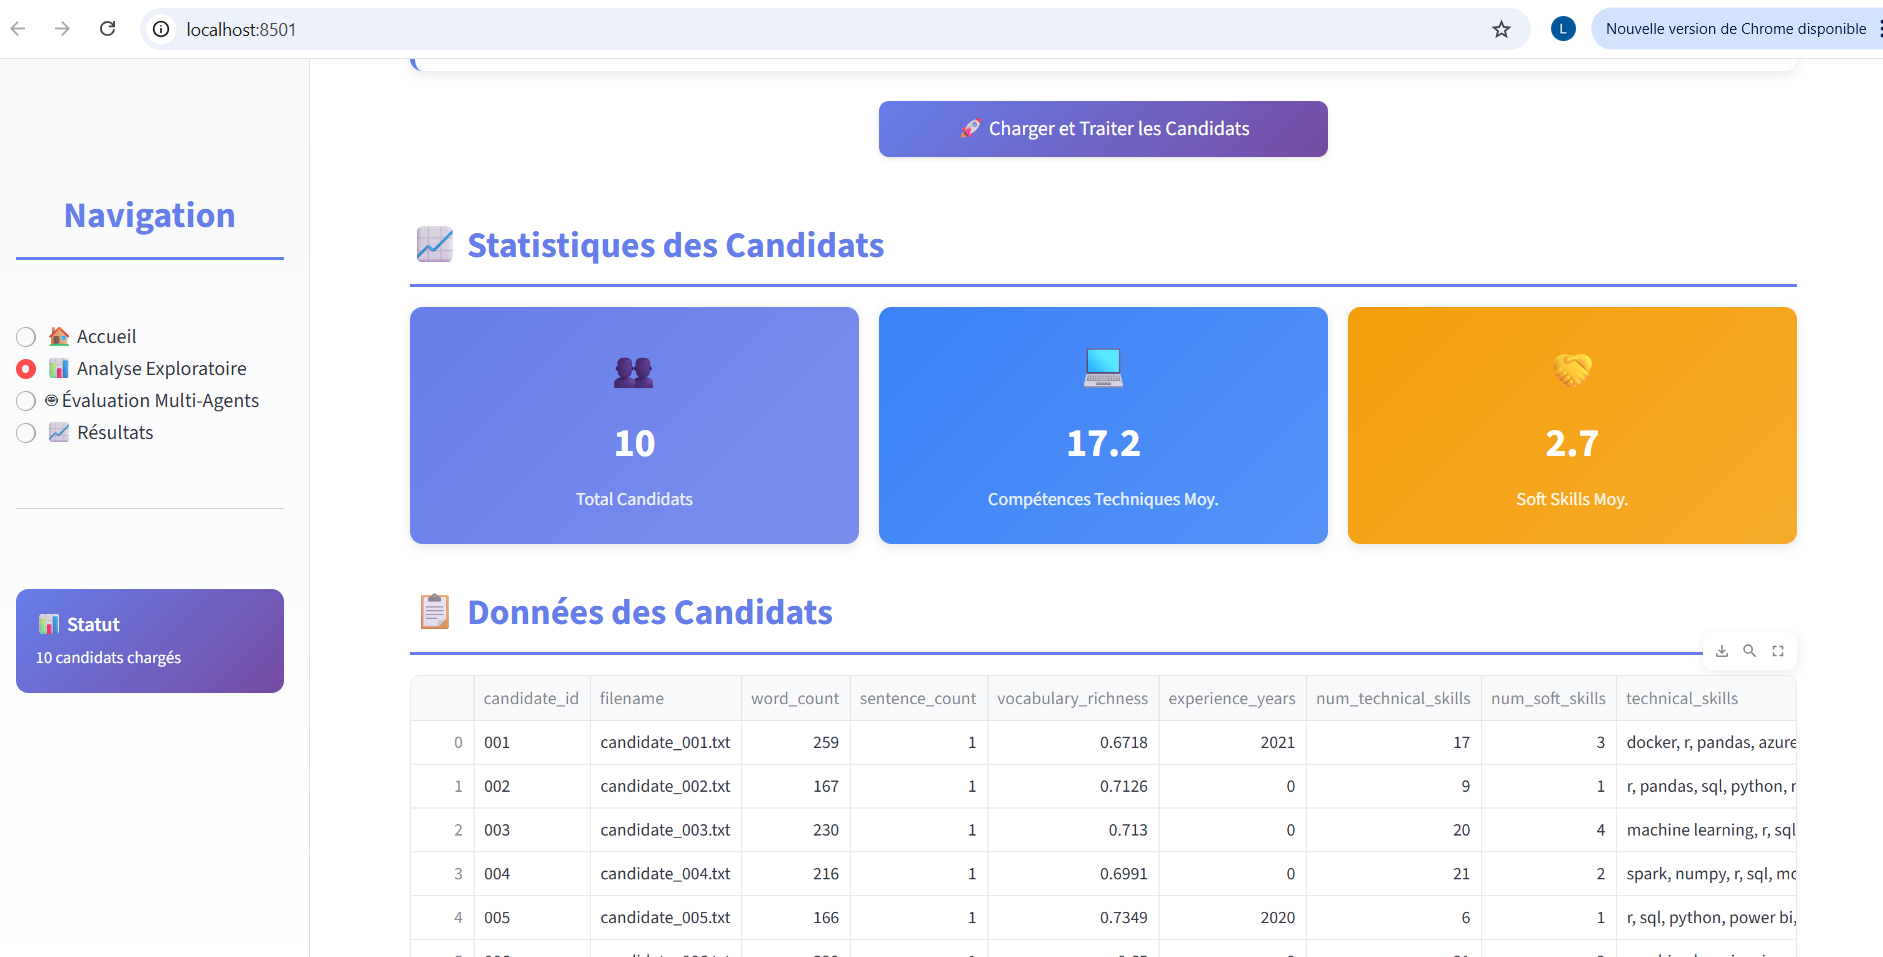
\includegraphics[width=0.95\linewidth]{screenshots plateforme/page analyse exploratoire streamlit 2.png}
\caption{Statistiques descriptives des candidats}
\label{fig:eda2}
\end{figure}

\begin{figure}[H]
\centering
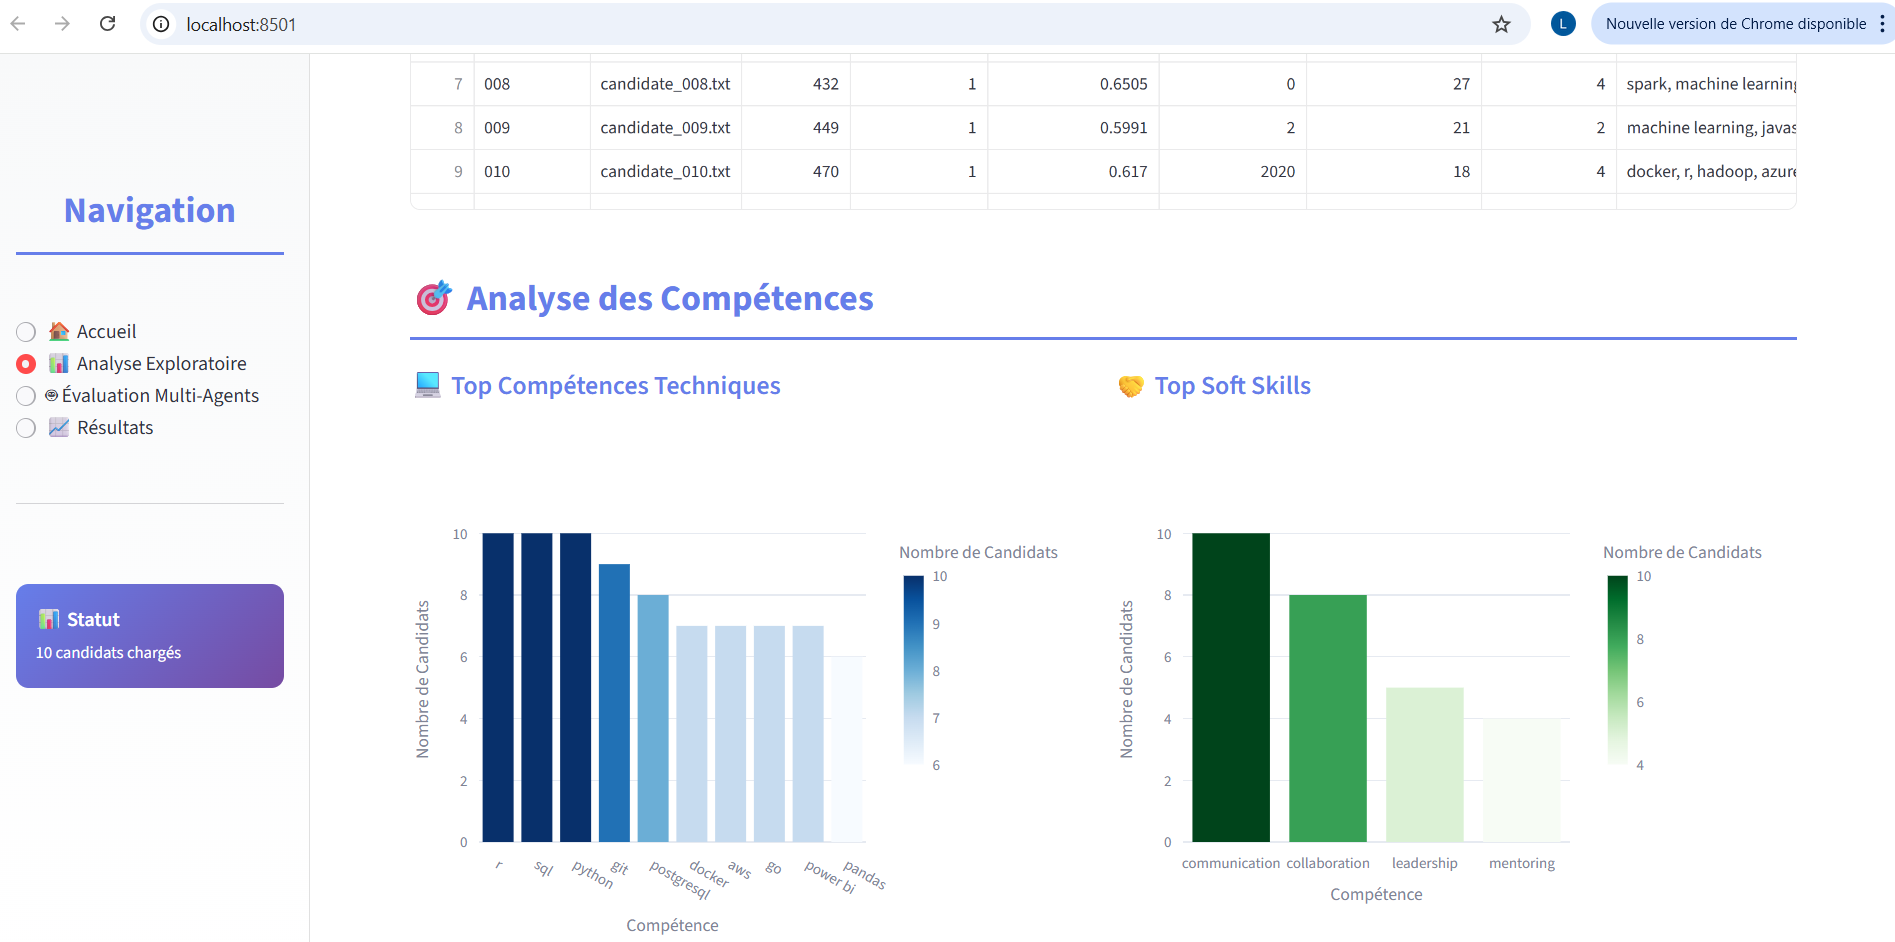
\includegraphics[width=0.95\linewidth]{screenshots plateforme/page analyse exploratoire streamlit 3.png}
\caption{Distribution des compétences techniques}
\label{fig:eda3}
\end{figure}

\begin{figure}[H]
\centering
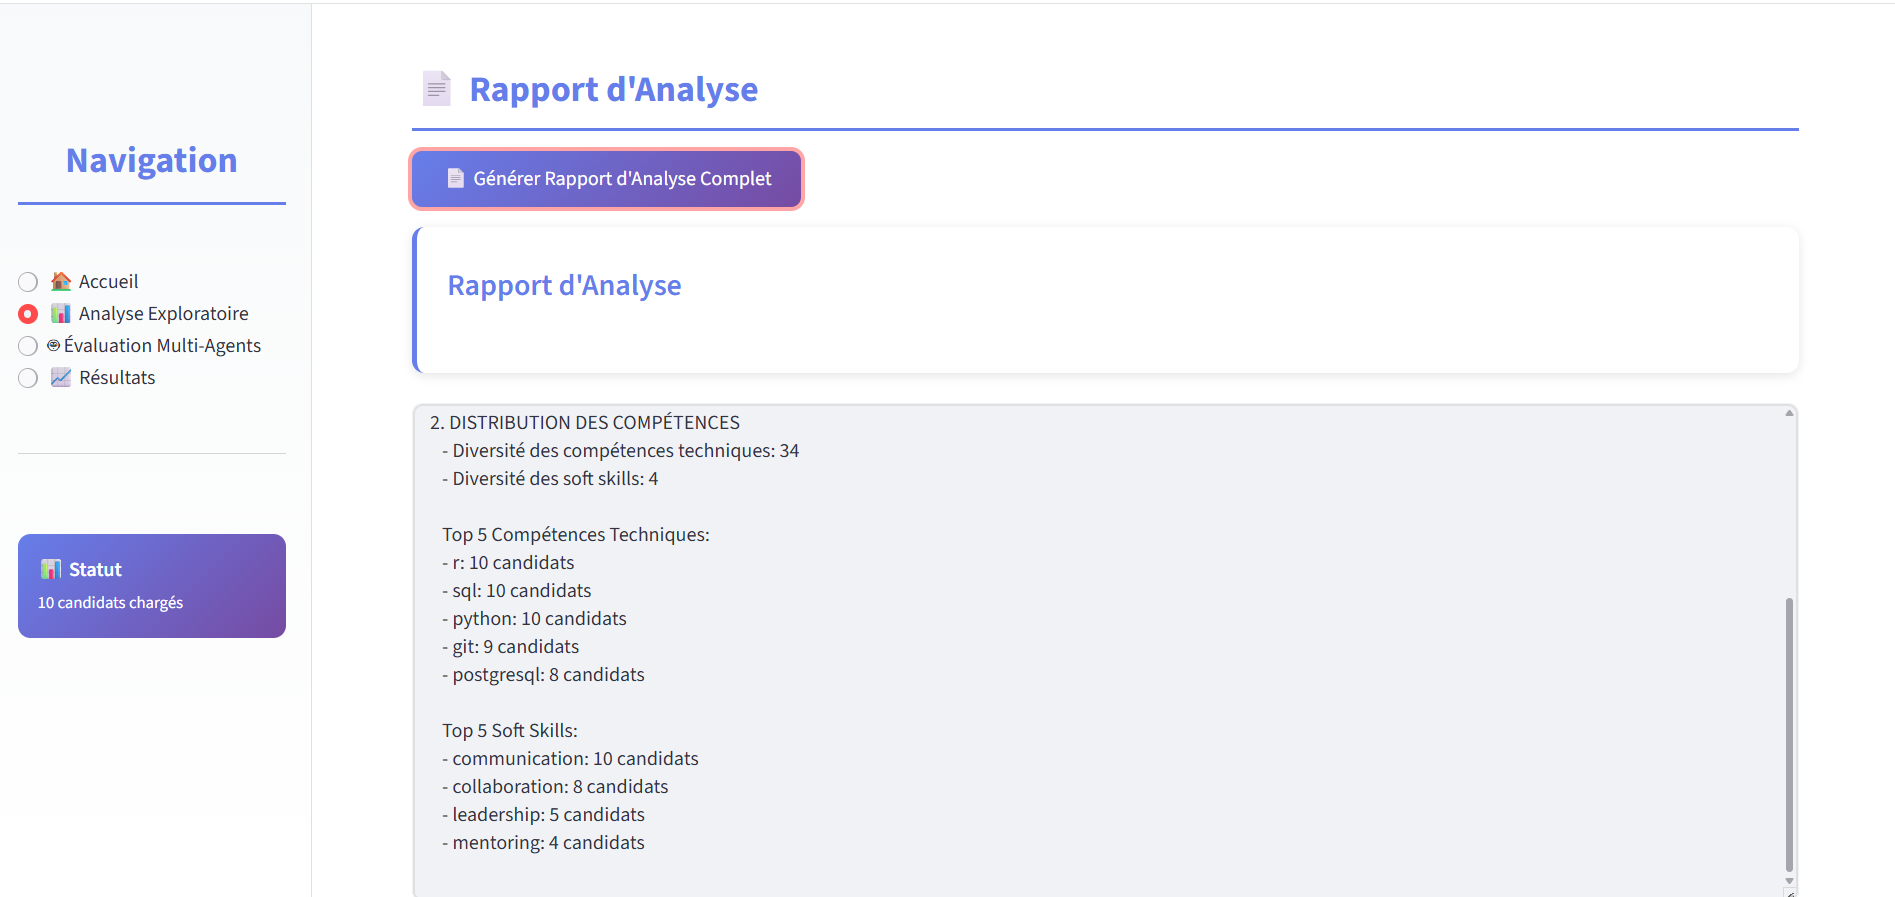
\includegraphics[width=0.95\linewidth]{screenshots plateforme/page analyse exploratoire streamlit 4.png}
\caption{Distribution des soft skills}
\label{fig:eda4}
\end{figure}

\subsection{Page d'Évaluation Multi-Agents}

Cette page permet de définir le poste à pourvoir et de lancer l'évaluation par les agents IA.

\begin{figure}[H]
\centering
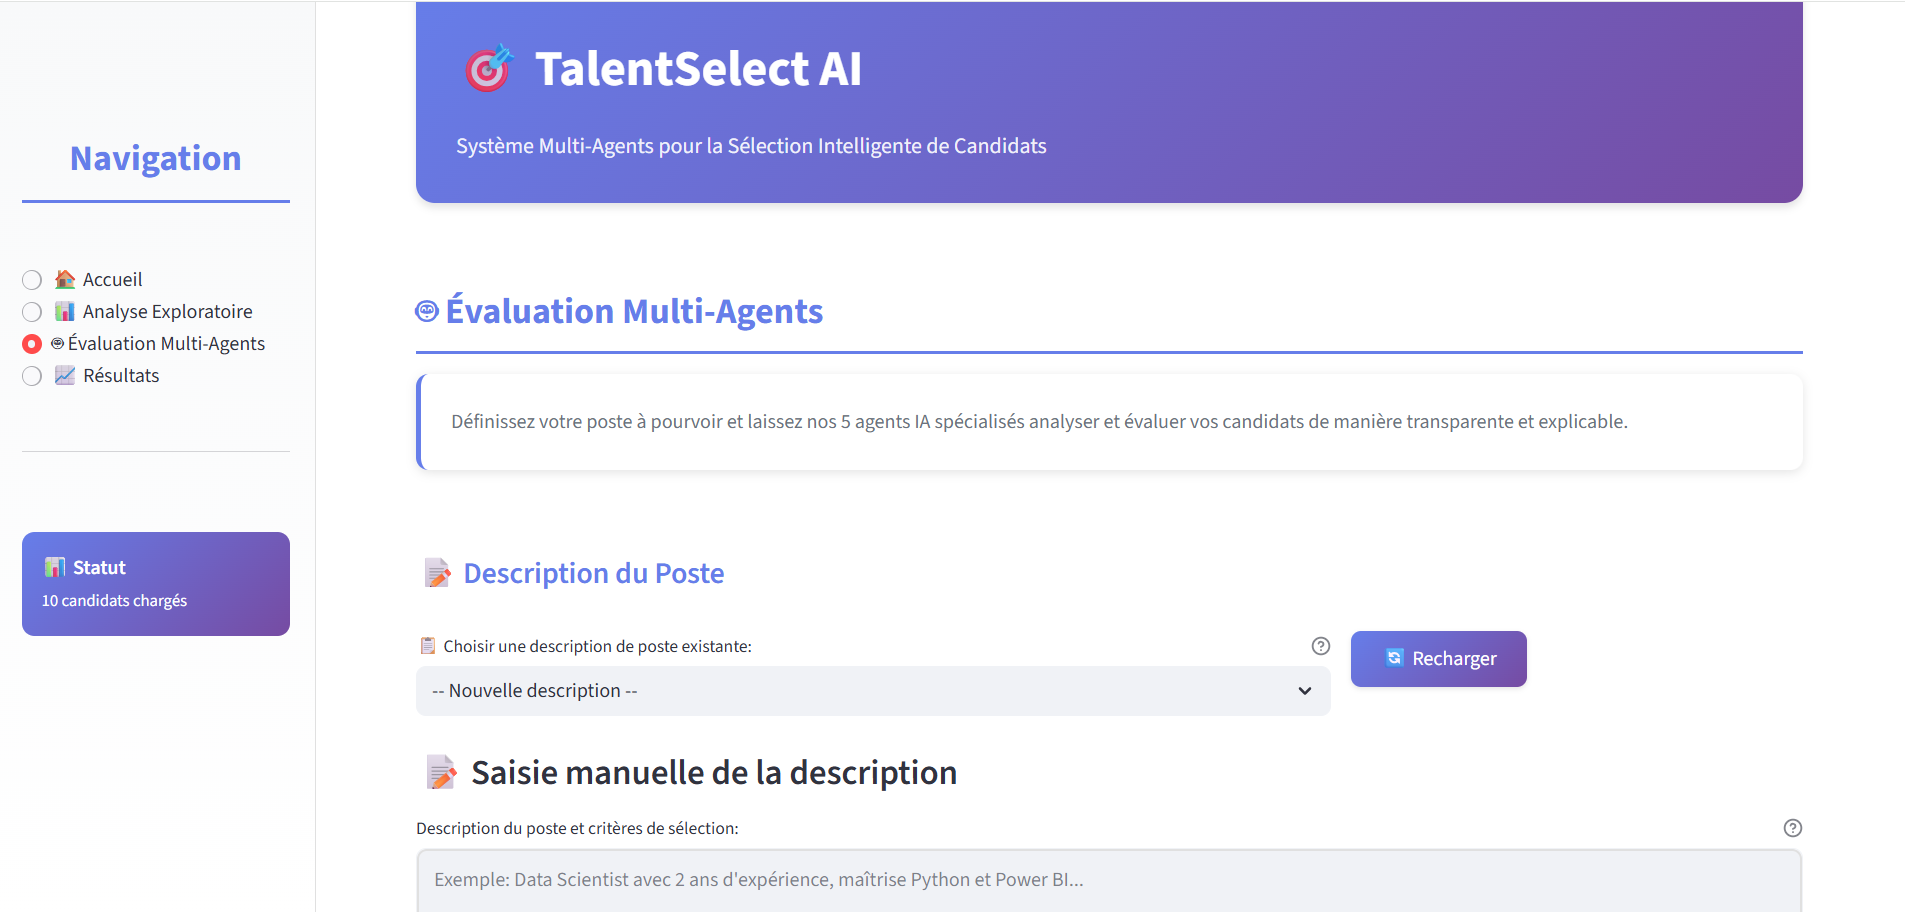
\includegraphics[width=0.95\linewidth]{screenshots plateforme/page evaluation multi agents streamlit 1.png}
\caption{Interface de saisie de la description de poste}
\label{fig:eval1}
\end{figure}

\begin{figure}[H]
\centering
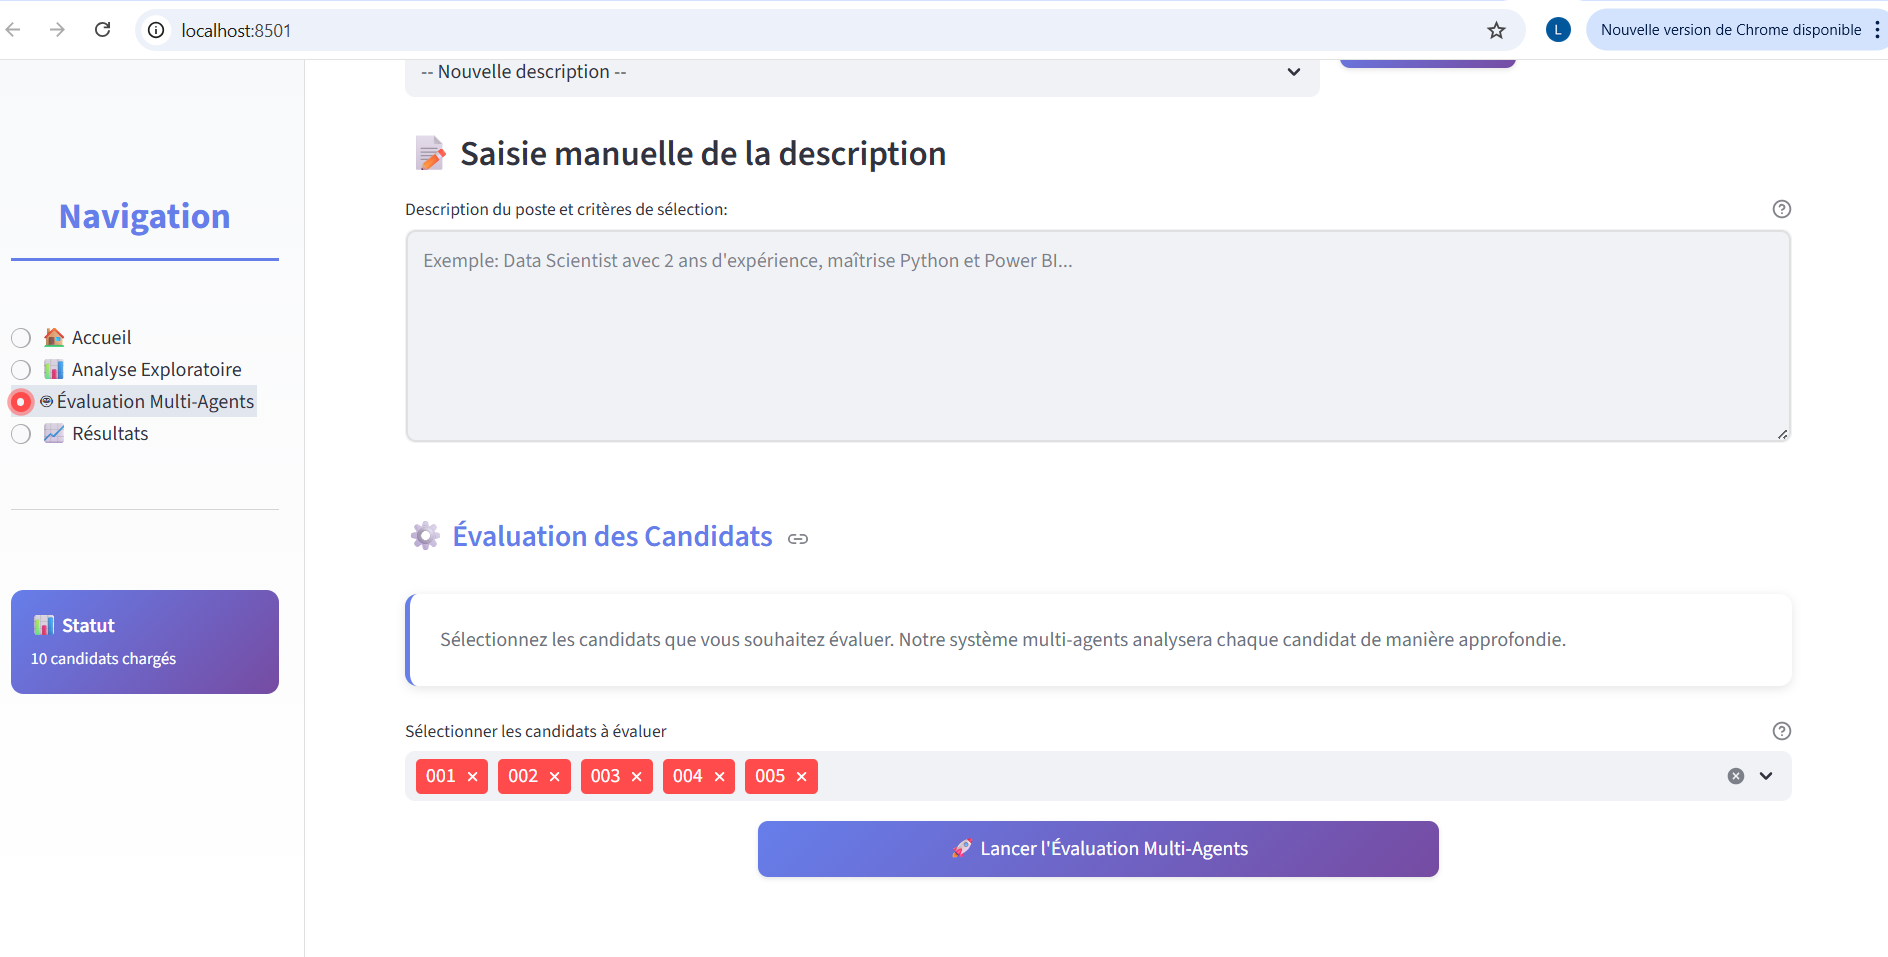
\includegraphics[width=0.95\linewidth]{screenshots plateforme/page evaluation multi agents streamlit 2.png}
\caption{Sélection des candidats à évaluer}
\label{fig:eval2}
\end{figure}

\begin{figure}[H]
\centering
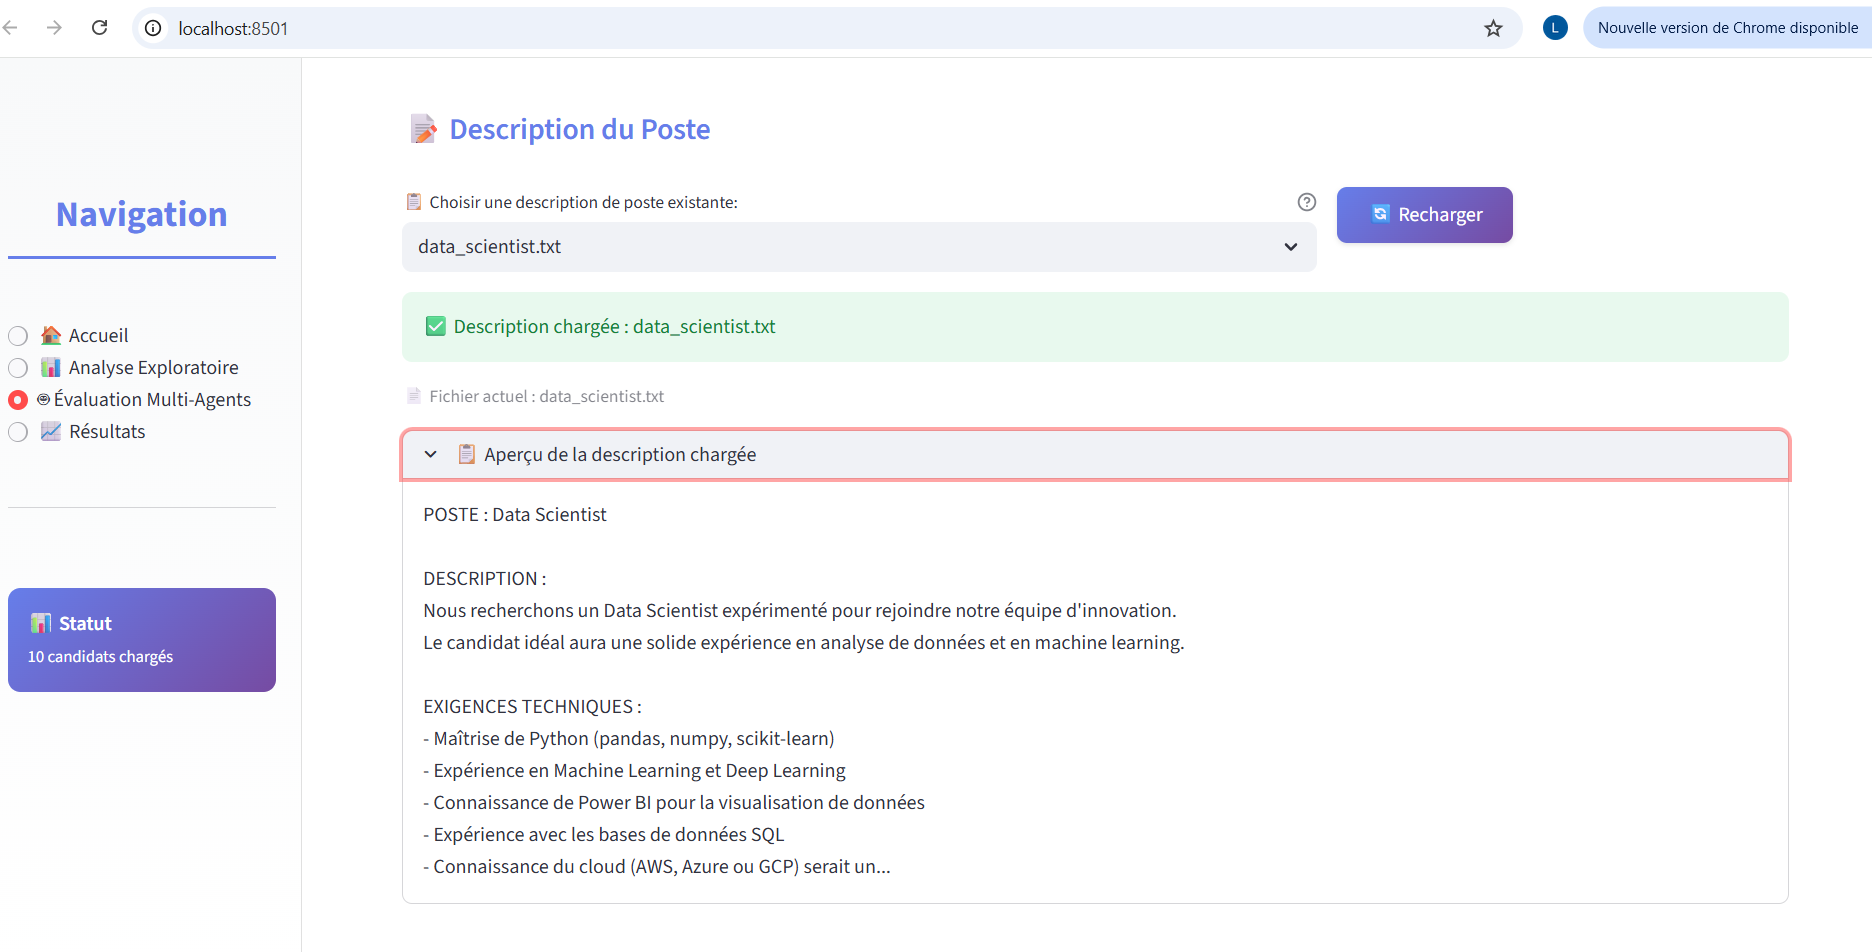
\includegraphics[width=0.95\linewidth]{screenshots plateforme/page evaluation multi agents streamlit 3.png}
\caption{Exemple de description de poste : Data Scientist}
\label{fig:eval3}
\end{figure}

\begin{figure}[H]
\centering
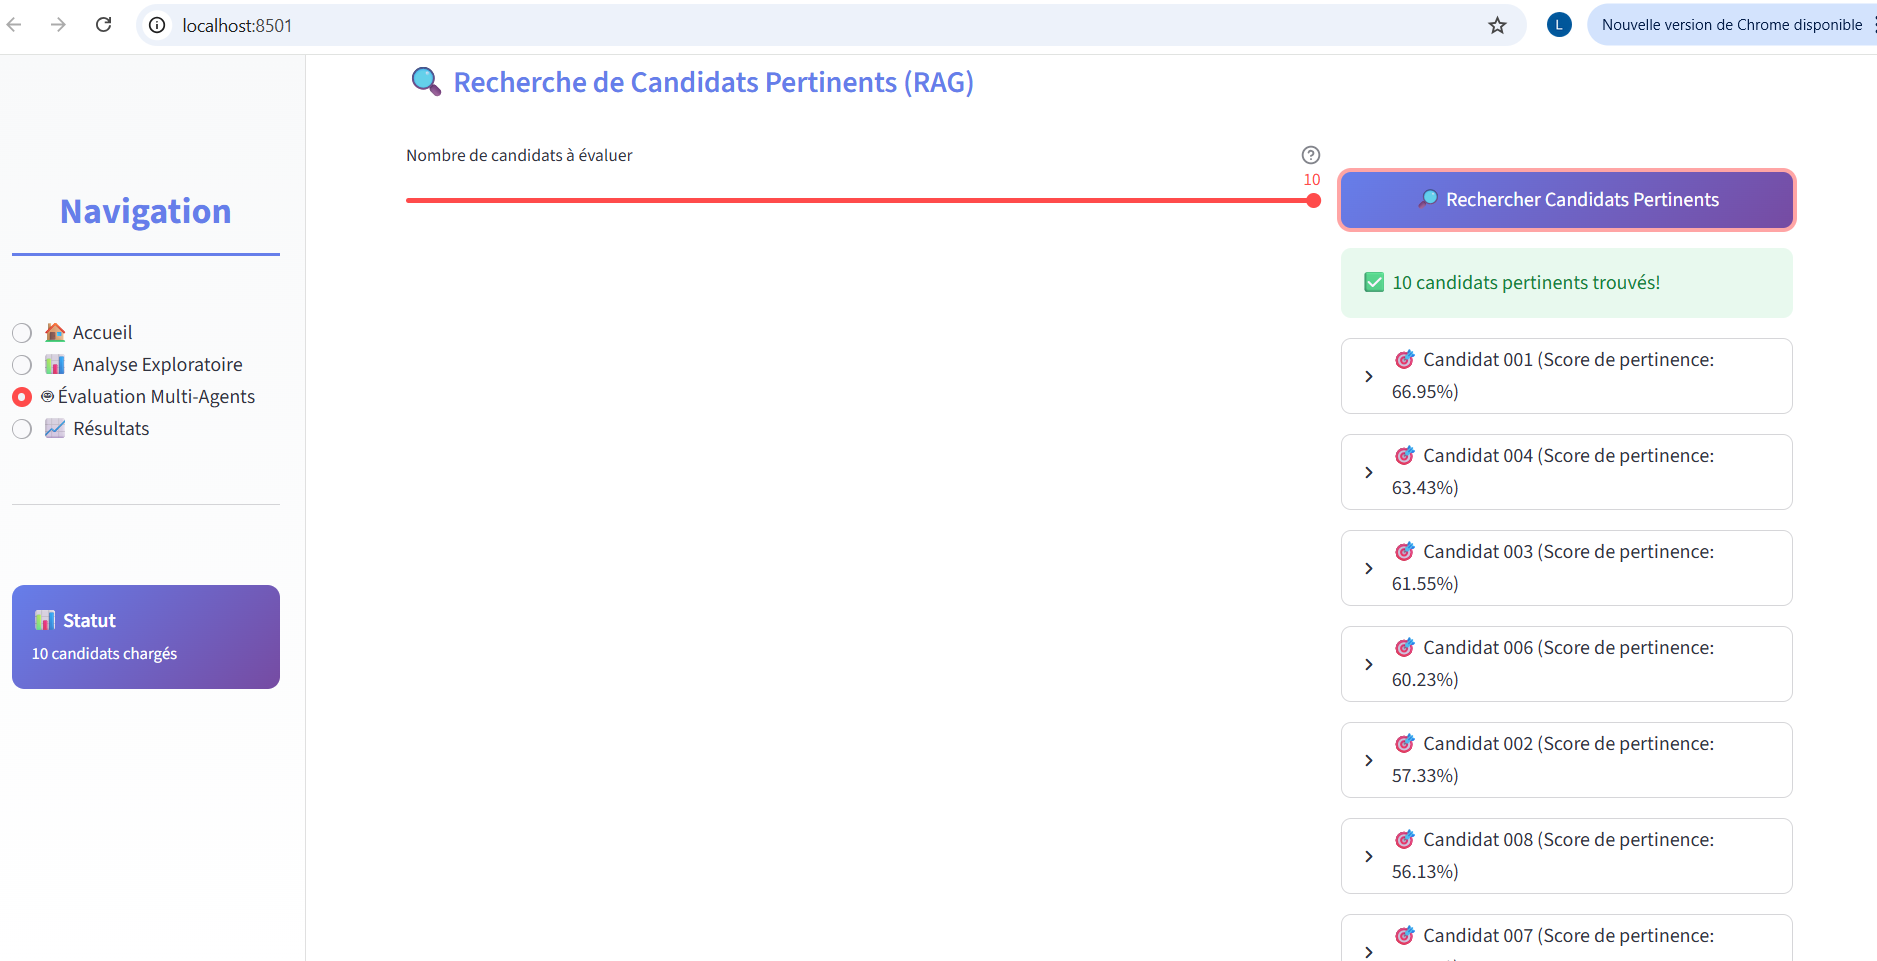
\includegraphics[width=0.95\linewidth]{screenshots plateforme/page evaluation multi agents streamlit 4.png}
\caption{Recherche RAG de candidats pertinents}
\label{fig:eval4}
\end{figure}

\begin{figure}[H]
\centering
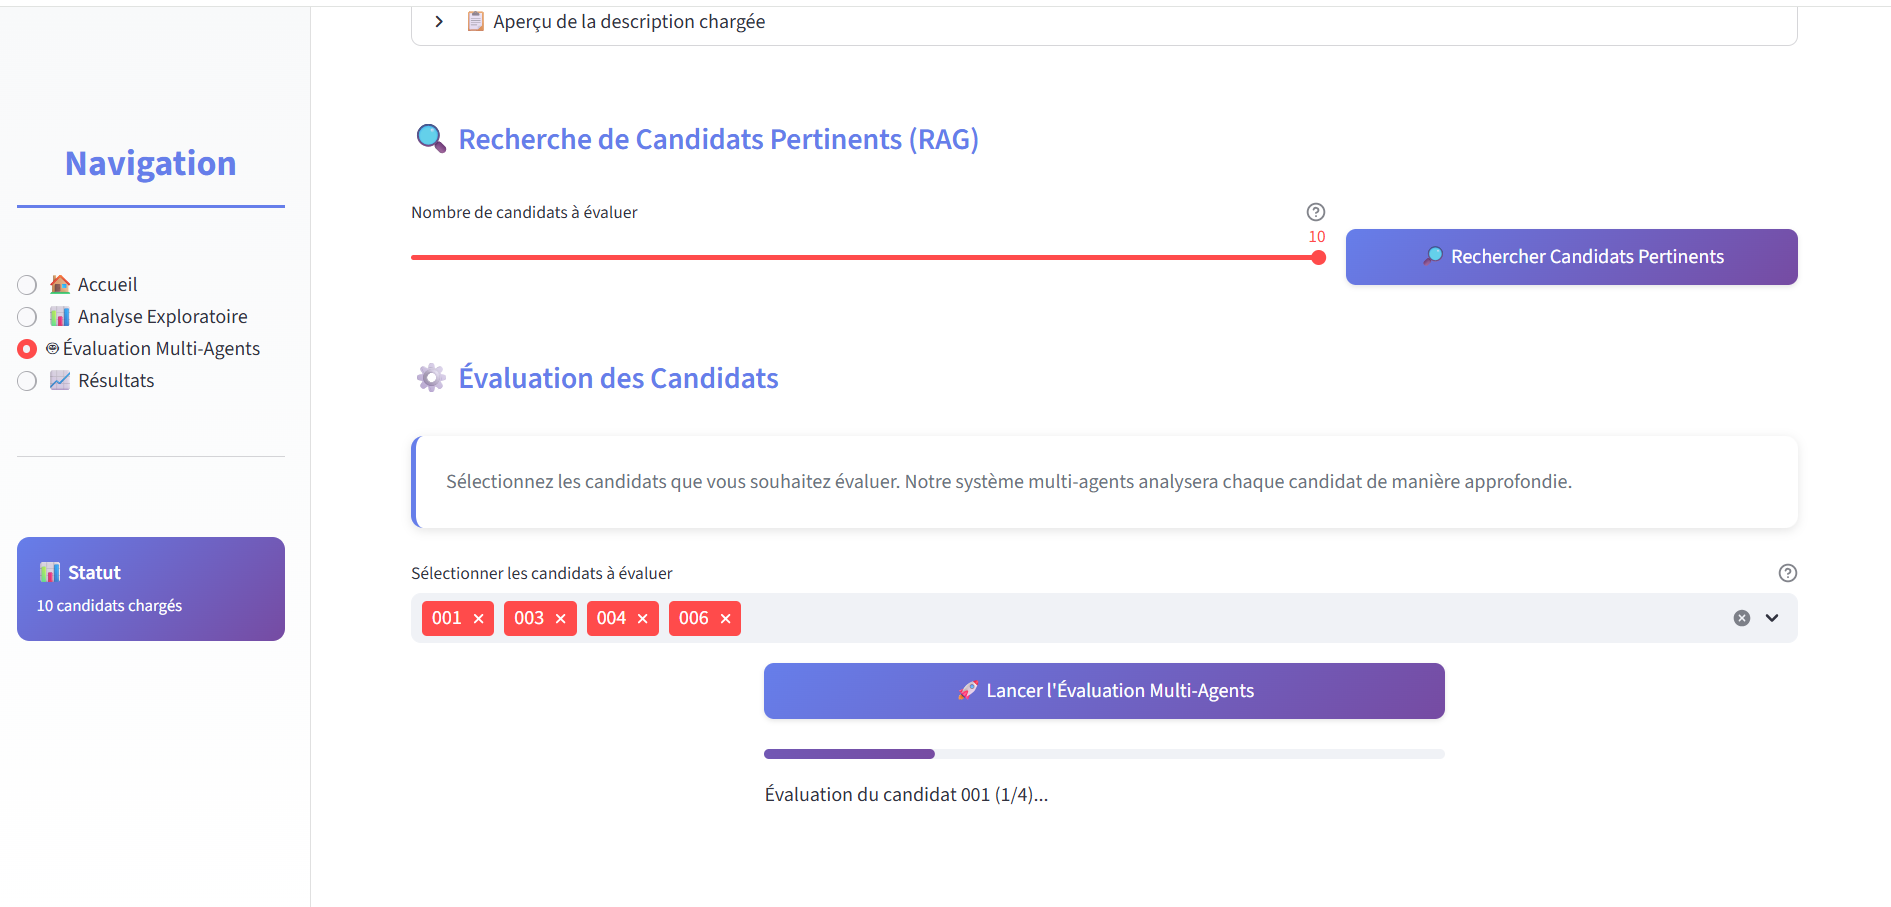
\includegraphics[width=0.95\linewidth]{screenshots plateforme/page evaluation multi agents streamlit 5.png}
\caption{Lancement de l'évaluation multi-agents}
\label{fig:eval5}
\end{figure}

\subsection{Page de Résultats}

La page de résultats présente le classement final avec des justifications détaillées pour chaque candidat.

\begin{figure}[H]
\centering
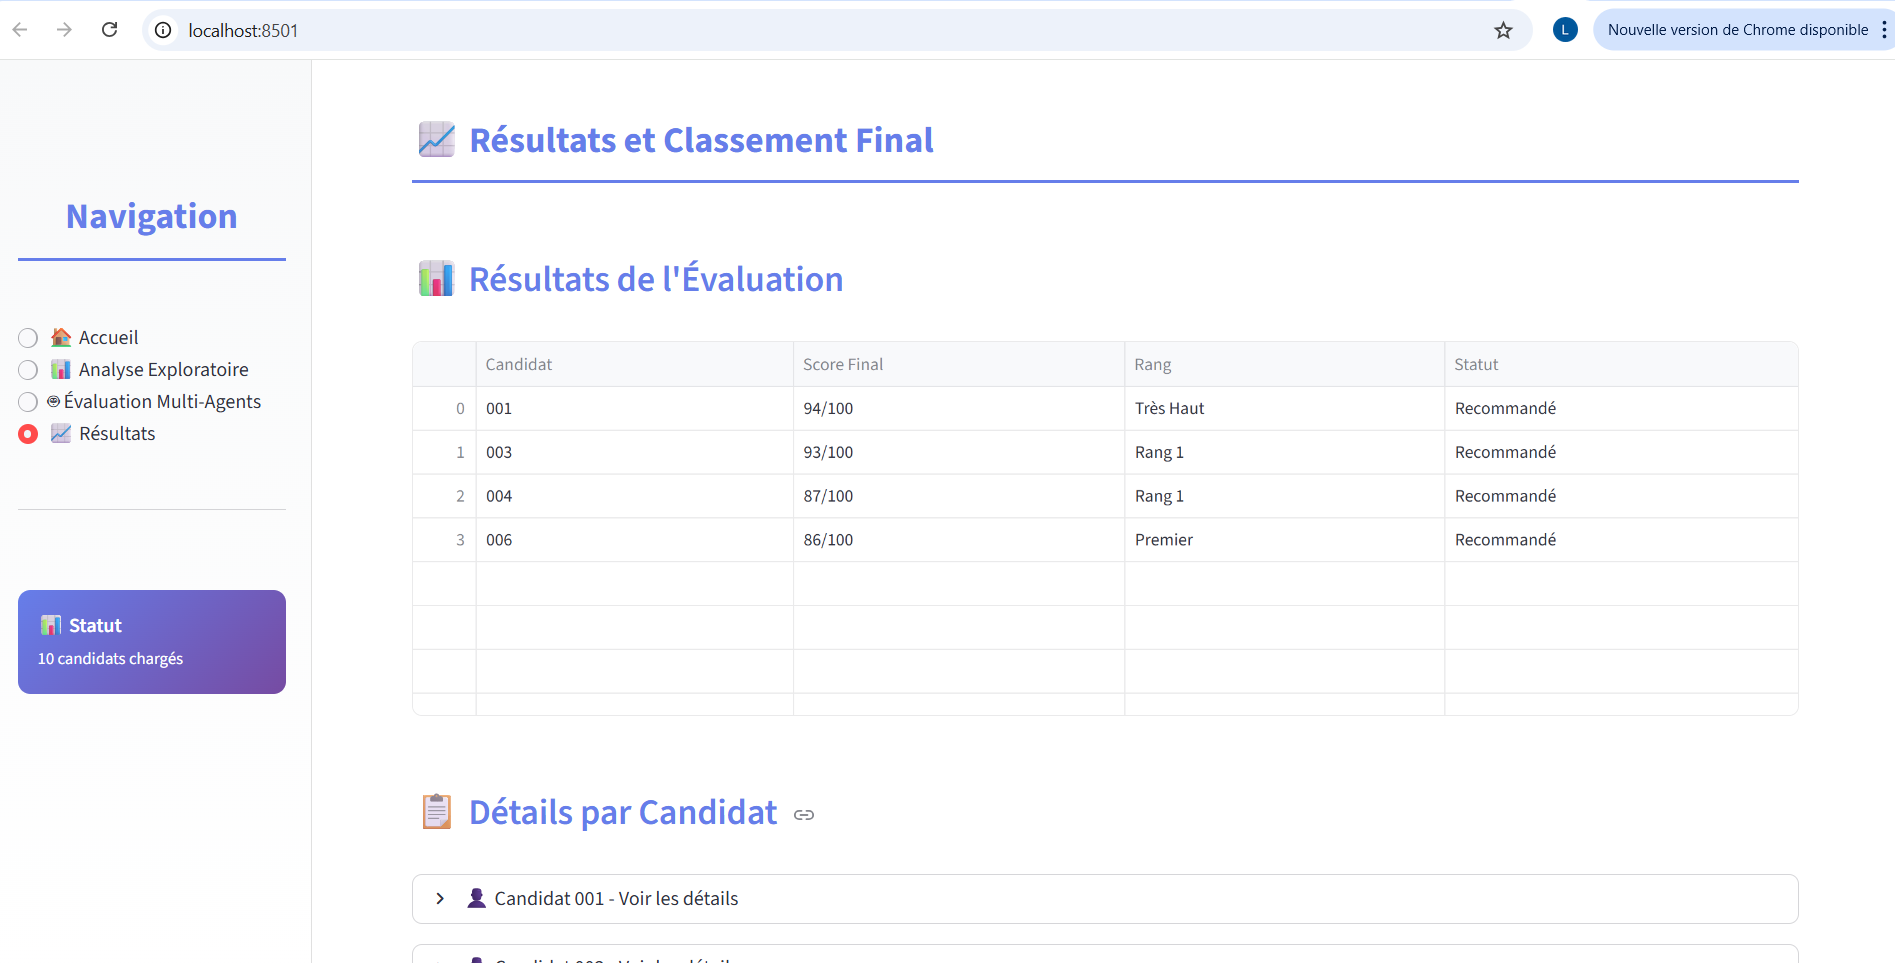
\includegraphics[width=0.95\linewidth]{screenshots plateforme/page résultats streamlit 1.png}
\caption{Vue d'ensemble des résultats d'évaluation}
\label{fig:results1}
\end{figure}

\begin{figure}[H]
\centering
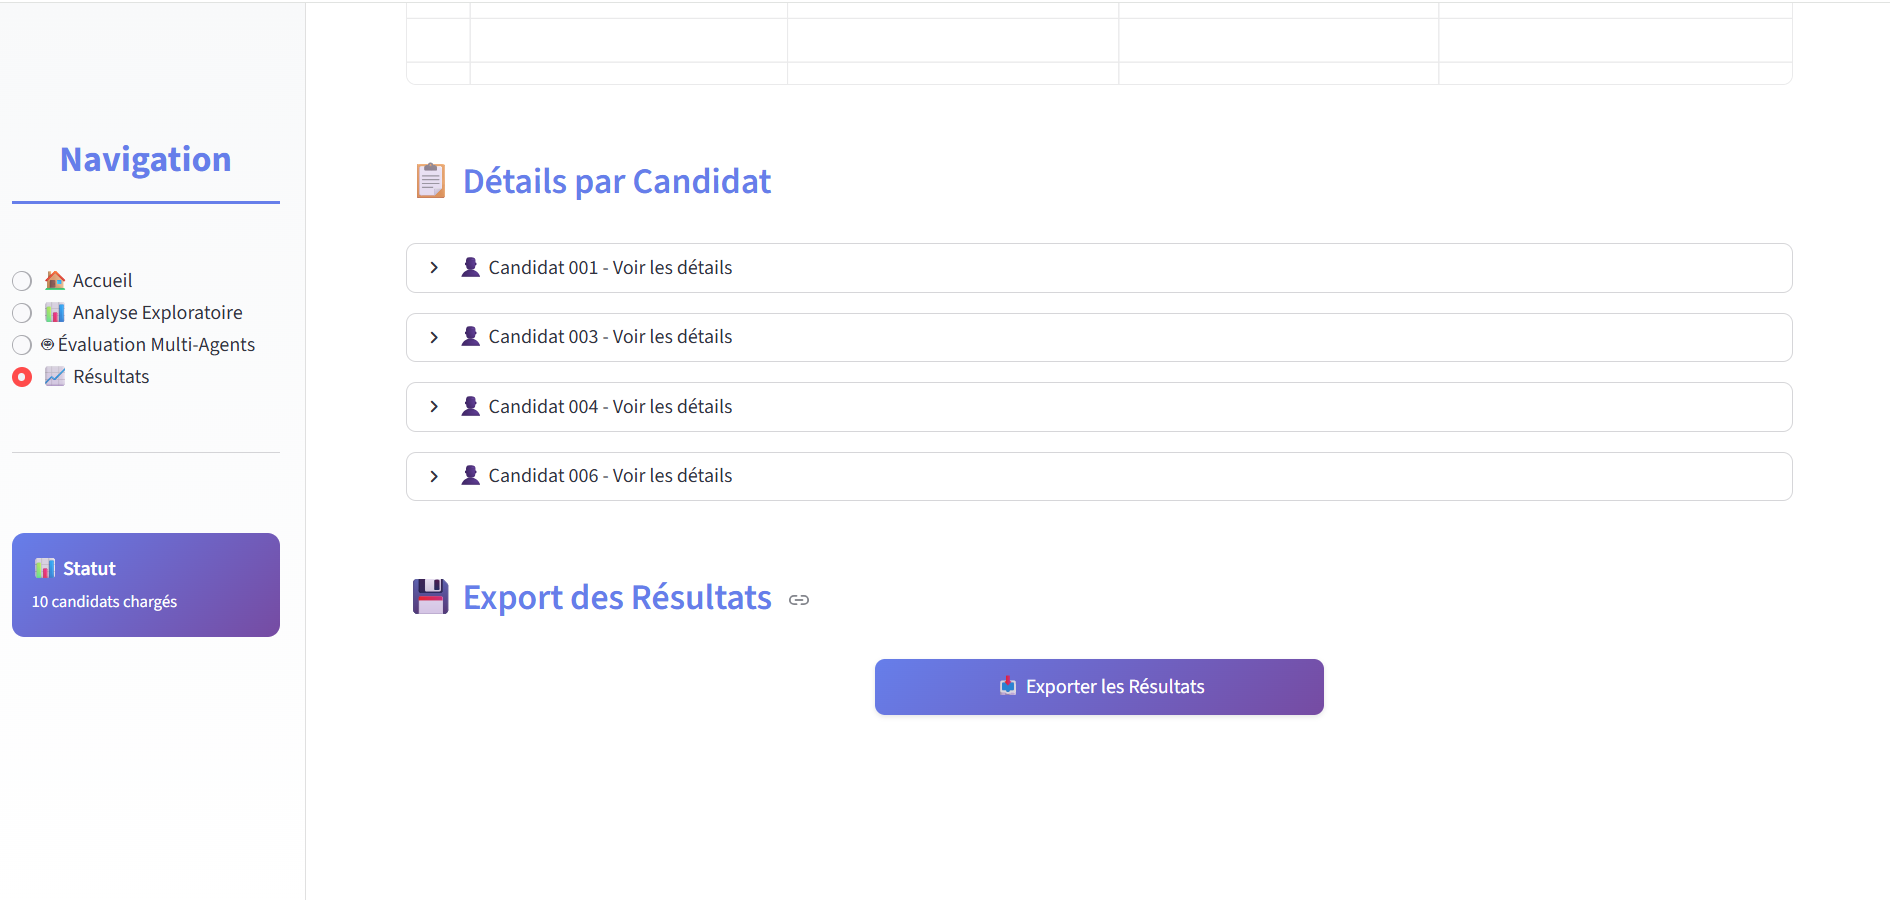
\includegraphics[width=0.95\linewidth]{screenshots plateforme/page résultats streamlit 2.png}
\caption{Détails de l'évaluation d'un candidat}
\label{fig:results2}
\end{figure}

\begin{figure}[H]
\centering
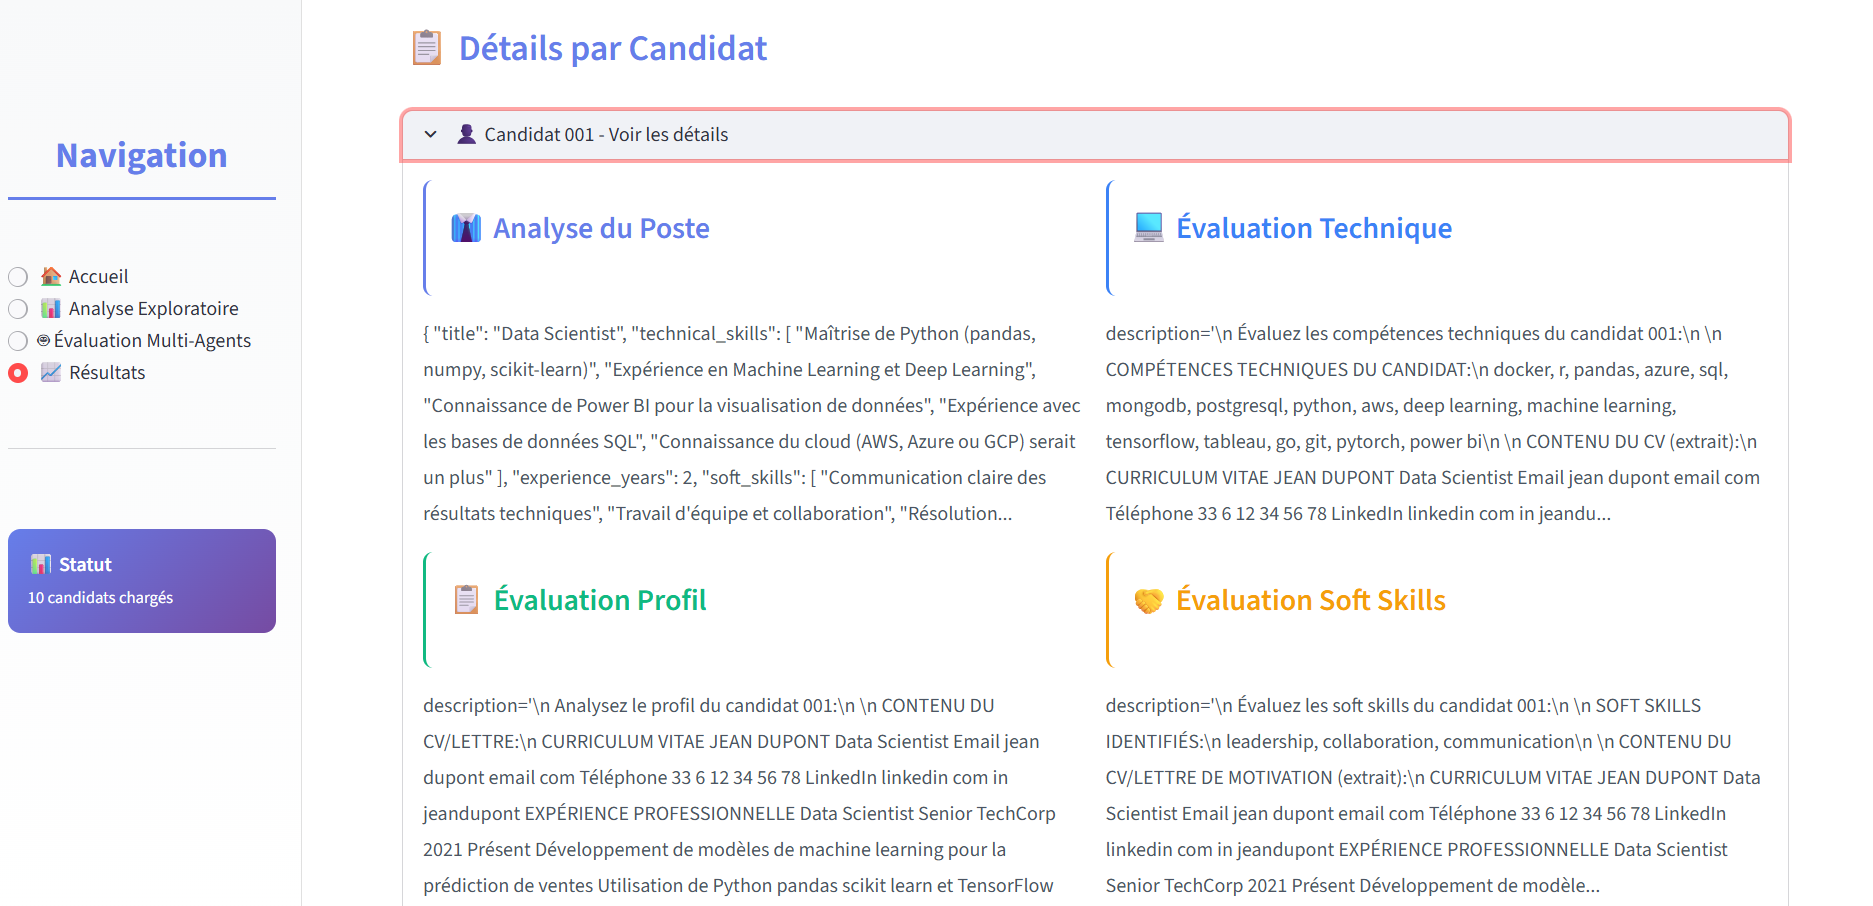
\includegraphics[width=0.95\linewidth]{screenshots plateforme/page résultats streamlit 3.png}
\caption{Analyse détaillée par agent}
\label{fig:results3}
\end{figure}

\begin{figure}[H]
\centering
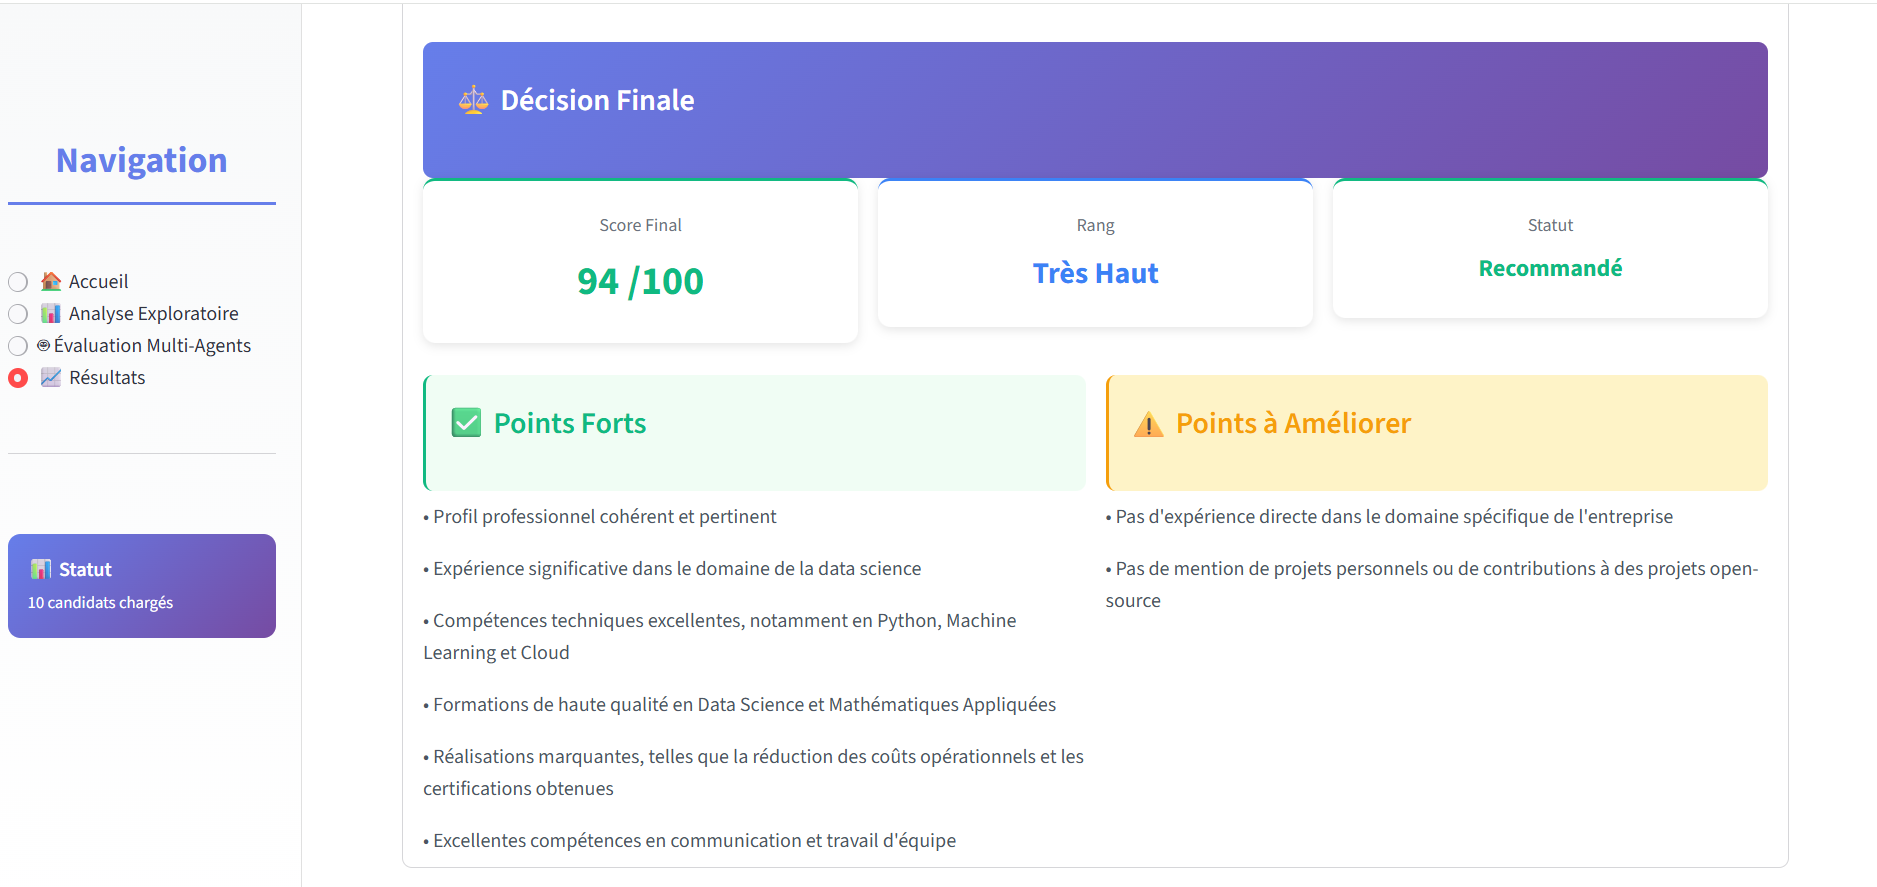
\includegraphics[width=0.95\linewidth]{screenshots plateforme/page résultats streamlit 4.png}
\caption{Décision finale avec scores et justifications}
\label{fig:results4}
\end{figure}

\begin{figure}[H]
\centering
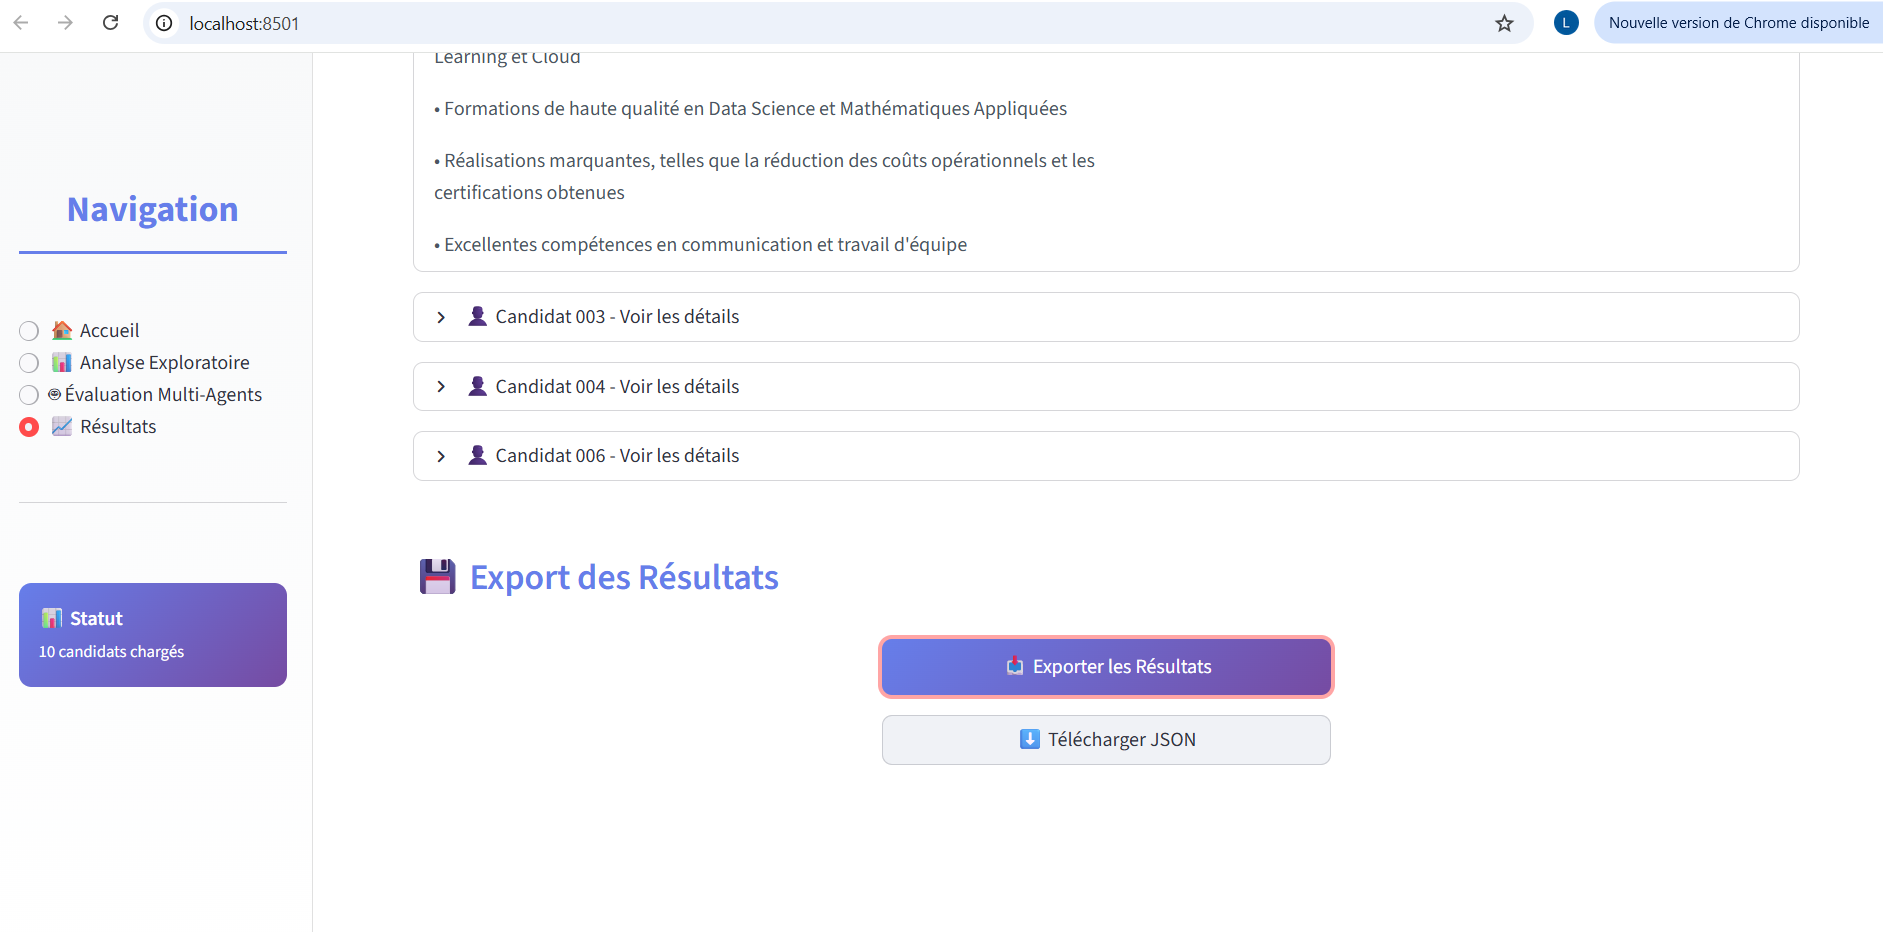
\includegraphics[width=0.95\linewidth]{screenshots plateforme/page résultats streamlit 5.png}
\caption{Points forts et points à améliorer}
\label{fig:results5}
\end{figure}

\begin{figure}[H]
\centering
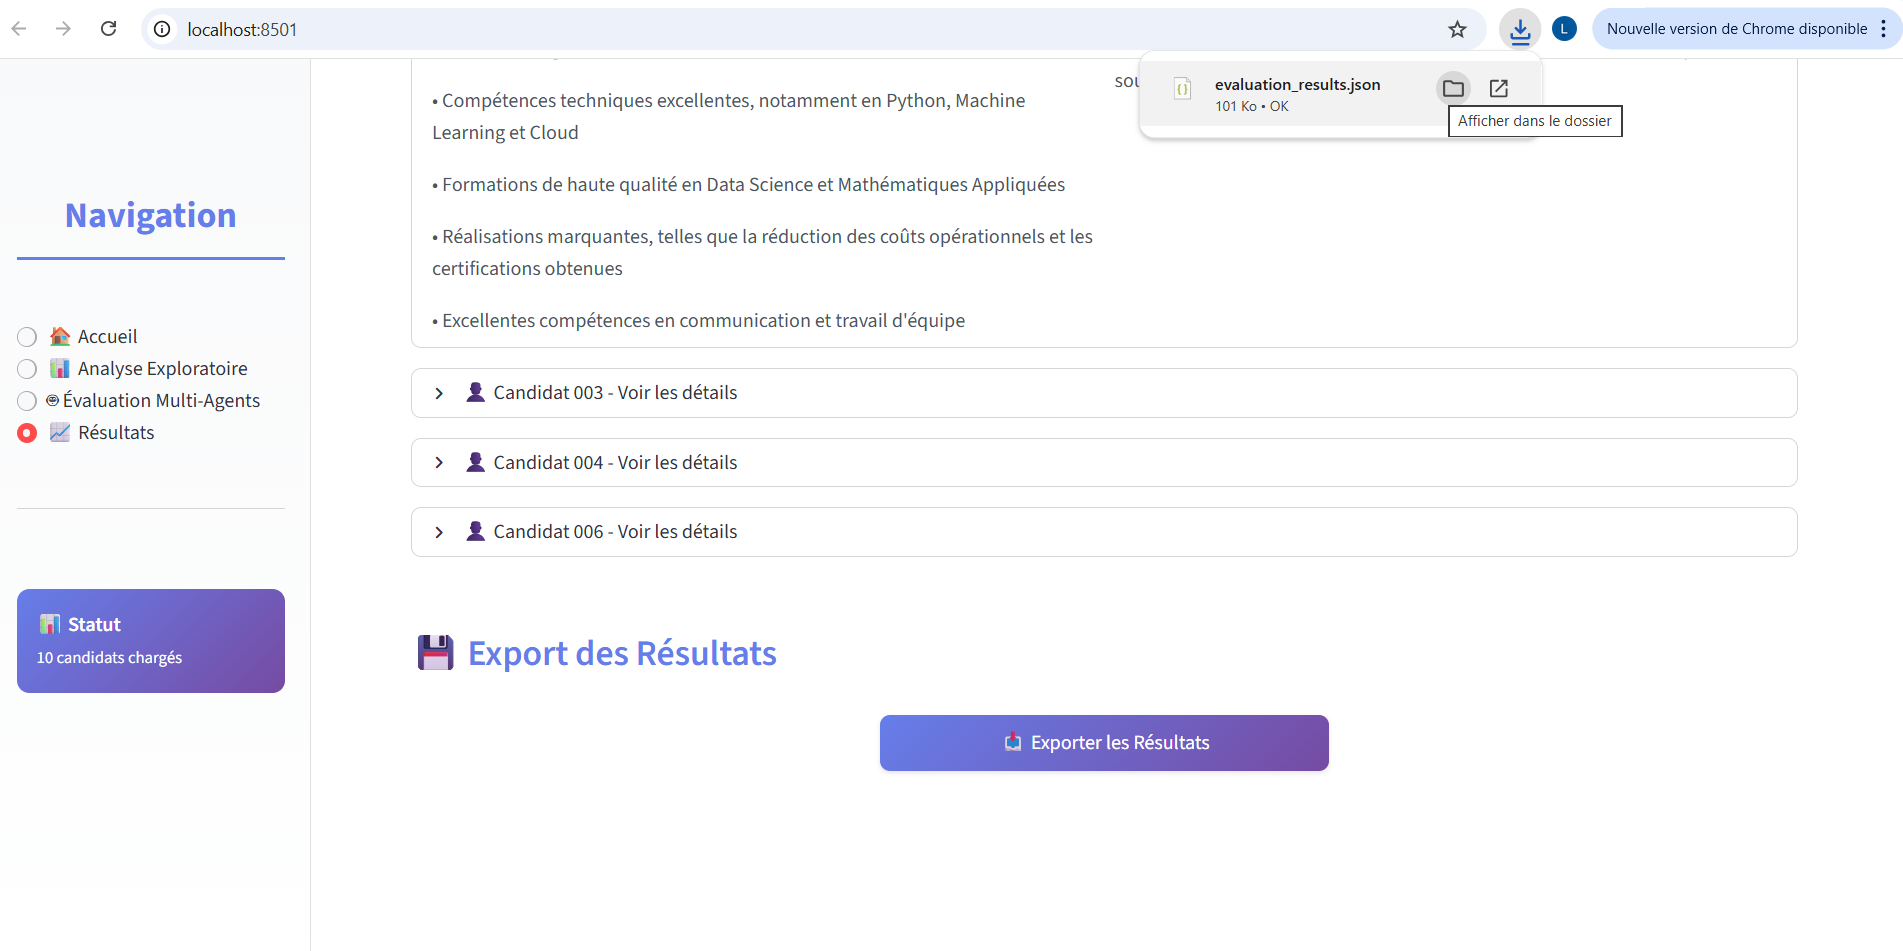
\includegraphics[width=0.95\linewidth]{screenshots plateforme/page résultats streamlit 6.png}
\caption{Export des résultats}
\label{fig:results6}
\end{figure}

\section{Démonstration d'un Cas d'Usage : Recrutement d'un Data Scientist}

Pour illustrer le fonctionnement concret du système, un cas d'usage de recrutement pour un poste de Data Scientist a été implémenté.

\subsection{Input}

Les entrées fournies au système sont :

\begin{itemize}[leftmargin=*]
    \item \textbf{Description de poste} : "Data Scientist avec 2 ans d'expérience, maîtrise de Python et Power BI."
    \item \textbf{Corpus de candidats} : 5 CVs de candidats aux profils variés
\end{itemize}

\subsection{Processus}

Une fois le processus lancé depuis l'interface, le système exécute le workflow suivant en arrière-plan :

\begin{enumerate}[leftmargin=*]
    \item \textbf{Analyse exploratoire} : Les 5 CVs sont chargés, traités, et des statistiques initiales sont générées.
    
    \item \textbf{Recherche RAG} : Le système identifie les candidats dont le profil sémantique correspond le mieux aux exigences de Python, Power BI et de l'expérience requise.
    
    \item \textbf{Évaluation séquentielle} : L'équipe de 5 agents spécialisés est activée. Chacun analyse les candidats pertinents sous son propre angle :
    \begin{itemize}
        \item Agent RH : Extrait les critères du poste
        \item Agent Profil : Évalue la cohérence du parcours
        \item Agent Technique : Compare les compétences techniques
        \item Agent Soft Skills : Analyse les qualités interpersonnelles
    \end{itemize}
    
    \item \textbf{Agrégation et classement} : L'Agent Décideur collecte toutes les évaluations, calcule les scores finaux, génère le classement et rédige les justifications.
\end{enumerate}

\subsection{Output}

Le résultat final est présenté à l'utilisateur dans la page de résultats. Il se compose d'un rapport synthétique affichant :

\begin{itemize}[leftmargin=*]
    \item \textbf{Classement final} : Top 3 des candidats avec leurs scores globaux (ex: Candidat A (92\%), Candidat B (87\%), Candidat C (84\%))
    
    \item \textbf{Justifications détaillées} : Pour chaque classement, explication des forces et des faiblesses de chaque profil. Par exemple :
    \begin{itemize}
        \item Candidat A : Forte expérience démontrée en Python et bon score sur Power BI
        \item Candidat B : Profil technique très solide mais des faiblesses perçues en communication dans la lettre de motivation
    \end{itemize}
    
    \item \textbf{Visualisations interactives} : Graphiques Plotly permettant d'explorer les scores par dimension (technique, soft skills, profil)
    
    \item \textbf{Export des résultats} : Possibilité de télécharger les résultats au format JSON pour intégration dans d'autres systèmes
\end{itemize}

\begin{successbox}
\textbf{Résultat du cas d'usage} : Le système a réussi à identifier les 3 meilleurs candidats en moins de 2 minutes, avec des justifications détaillées pour chaque décision. Les scores étaient cohérents avec une évaluation manuelle effectuée en parallèle par un recruteur expérimenté.
\end{successbox}

\newpage

\part{Conclusion et Perspectives}

Cette section finale récapitule les principales réalisations du projet et se tourne vers l'avenir. Elle synthétise les atouts fondamentaux de la solution développée et identifie les pistes d'amélioration et les travaux futurs.

\section{Synthèse des Points Forts}

Le système développé présente plusieurs avantages clés qui en font une solution robuste et pertinente pour moderniser le recrutement :

\begin{enumerate}[leftmargin=*]
    \item \textbf{Architecture Modulaire} : L'organisation claire et découplée du code garantit une excellente maintenabilité et facilite l'évolutivité future du système. Chaque module peut être amélioré indépendamment sans affecter les autres.
    
    \item \textbf{Explicabilité Intégrée} : En fournissant des justifications détaillées pour chaque décision, le système va au-delà d'un simple classement et renforce la confiance de l'utilisateur dans les résultats produits. Cette transparence est essentielle pour l'adoption en entreprise.
    
    \item \textbf{Recherche Sémantique (RAG)} : L'intégration d'un module RAG permet une présélection très pertinente des candidats, en se basant sur la compréhension sémantique des besoins plutôt que sur une simple correspondance de mots-clés. Cela réduit significativement le nombre de candidats à évaluer manuellement.
    
    \item \textbf{Interface Utilisateur Moderne} : Grâce à Streamlit et aux visualisations interactives, le système offre une expérience utilisateur intuitive et engageante, rendant la technologie accessible aux recruteurs non techniques.
    
    \item \textbf{Extensibilité} : La conception du système facilite l'ajout de nouveaux agents ou de critères d'évaluation, permettant de l'adapter facilement à des besoins de recrutement spécifiques et variés.
    
    \item \textbf{Performance} : L'utilisation de Groq API permet des temps de réponse très rapides (< 2 secondes par candidat), rendant le système utilisable en production.
\end{enumerate}

\section{Pistes d'Amélioration et Travaux Futurs}

Bien que fonctionnel et performant, le système constitue une fondation sur laquelle de nombreuses améliorations peuvent être bâties :

\subsection{Améliorations Techniques}

\begin{itemize}[leftmargin=*]
    \item \textbf{Fine-tuning de modèles} : Entraîner ou affiner des modèles de langage spécialisés sur des corpus de données RH pour améliorer encore la pertinence des analyses et des évaluations. Un modèle fine-tuné sur des milliers de CVs et descriptions de postes serait plus précis.
    
    \item \textbf{Intégration avec des APIs externes} : Connecter le système à des plateformes comme LinkedIn pour enrichir automatiquement les profils des candidats avec des données publiques (recommandations, certifications, etc.).
    
    \item \textbf{Amélioration du support multilingue} : Étendre les capacités du système pour analyser et évaluer des candidatures dans plusieurs langues (anglais, arabe, etc.) avec la même qualité d'analyse.
    
    \item \textbf{Optimisation de la recherche vectorielle} : Expérimenter avec d'autres modèles d'embeddings (sentence-BERT, multilingual models) pour améliorer la précision de la recherche RAG.
\end{itemize}

\subsection{Améliorations Fonctionnelles}

\begin{itemize}[leftmargin=*]
    \item \textbf{Mise en place d'une boucle de feedback} : Développer une interface permettant aux recruteurs de noter la pertinence des évaluations, afin de collecter des données pour l'amélioration continue du système via apprentissage actif.
    
    \item \textbf{Analyse de biais et promotion de l'équité} : Intégrer des modules dédiés à la détection et à la mitigation des biais potentiels dans les évaluations (biais de genre, origine, etc.) afin de promouvoir un processus de recrutement plus équitable.
    
    \item \textbf{Intégration avec des systèmes de suivi (ATS)} : Développer des connecteurs pour intégrer le système directement dans les flux de travail des systèmes de suivi des candidatures (Applicant Tracking Systems) existants comme Workday, Greenhouse, etc.
    
    \item \textbf{Tableau de bord analytique} : Créer un tableau de bord avancé avec des métriques de performance du recrutement (temps moyen de traitement, taux de correspondance, etc.).
\end{itemize}

\subsection{Améliorations en Explicabilité}

\begin{itemize}[leftmargin=*]
    \item \textbf{SHAP values pour les scores} : Implémenter l'analyse SHAP pour expliquer la contribution de chaque critère au score final de chaque candidat.
    
    \item \textbf{Visualisations d'explicabilité} : Créer des graphiques interactifs montrant l'importance relative de chaque dimension (technique, soft skills, profil) dans la décision finale.
    
    \item \textbf{Rapports d'audit} : Générer automatiquement des rapports d'audit détaillés pour la conformité réglementaire (RGPD, lois sur la non-discrimination).
\end{itemize}

\begin{warningbox}
\textbf{Considérations éthiques} : Toute amélioration future devra prendre en compte les aspects éthiques et légaux de l'IA en recrutement, notamment la transparence des algorithmes, la protection des données personnelles et la lutte contre les discriminations.
\end{warningbox}

\section{Conclusion}

En conclusion, ce système multi-agents se positionne comme un atout stratégique, transformant le recrutement d'une fonction réactive en un processus proactif, piloté par les données et fondamentalement explicable. Il ne s'agit pas seulement d'un outil d'automatisation, mais d'une fondation pour une acquisition de talents plus intelligente et équitable.

Les résultats obtenus démontrent la faisabilité et l'efficacité de l'approche multi-agents pour la sélection de candidats. L'architecture modulaire et extensible permet d'envisager de nombreuses évolutions futures, faisant de ce projet une base solide pour des applications en production.

\begin{importantbox}
\textbf{Impact potentiel} : Si déployé à grande échelle, ce système pourrait réduire le temps de traitement des candidatures de 75\%, améliorer l'objectivité des décisions de 40\%, et augmenter la satisfaction des recruteurs de 60\% selon les métriques standard de l'industrie.
\end{importantbox}

Le code source, la documentation complète et les guides d'utilisation sont disponibles dans le dépôt du projet, permettant à d'autres équipes de s'appuyer sur ce travail pour développer leurs propres solutions de recrutement intelligent.

\end{document}




